\documentclass[french,nolocaltoc]{nwejmart}
\usepackage{denisbdoc}
\usepackage{draftwatermark}
\usepackage{embedfile}
%
\indexsetup{level=\section*,toclevel=section,noclearpage}
\makeindex[columns=2]
\tcbset{index format=off}
%
\lstMakeShortInline[style=dbtex]|
\tcbset{listing options={escapechar=+}}
%
% \ExplSyntaxOn
\makeatletter
\renewcommand{\thetcb@cnt@dbremark}{\arabic{tcb@cnt@dbremark}}%
\renewcommand{\thetcb@cnt@dbwarning}{\arabic{tcb@cnt@dbwarning}}%
\renewcommand{\thetcb@cnt@dbexample}{\arabic{tcb@cnt@dbexample}}%
\renewcommand{\thetcb@cnt@dbfaq}{\arabic{tcb@cnt@dbfaq}}%
% \clist_set:Nn \l_tmpa_clist {dbremark}
% \clist_map_inline:Nn \l_tmpa_clist {
%   \renewcommand{\thetcb@cnt@##1}{\arabic{tcb@cnt@##1}}%
% }
\makeatother
% \ExplSyntaxOff
%
\SetWatermarkColor{gray!10}%
\SetWatermarkFontSize{20mm}%
\SetWatermarkText{\MakeUppercase{travail en cours}}%
%
\addbibresource{nwejm.bib}
%
\newacronym{nwejm}{nwejm}{North-Western European Journal of Mathematics}
\newacronym{bap}{bap}{bounded approximation property}
\newacronym{msc}{msc}{Mathematical Subject Classification}
\newacronym{url}{url}{Uniform Resource Locator}
%
\newtheorem{article}
\newtheorem[title=Fait,style=definition]{fact}
%
\DeclareMathOperator{\cat}{Cat}
\newcommand{\mybinop}{\mathbin{@}}
%
\begin{document}
\title[Documentation de la classe \LaTeX{} du \texorpdfstring{\nwejm}{NWEJM}]{Documentation de la classe \LaTeX{} du \nwejm*{} destinée aux auteurs}
%
\author[%
affiliation={%
  Université du Littoral Côte d'Opale, Laboratoire de mathématiques pures et
  appliquées (\nolinkurl{denis.bitouze@lmpa.univ-littoral.fr})%
},%
]{Bitouzé, Denis}
%
\maketitle
%
\etocarticlestylenomarks
\localtableofcontents
%
\DeclareFixedFootnote{\conseilslatex}{Et donne de façon subliminale quelques conseils
  \LaTeX{}. On consultera \autocite{Ensenbach} pour un panorama plus complet des
  commandes et extensions obsolètes (et autres erreurs).}

%%% Local Variables:
%%% mode: latex
%%% TeX-master: "nwejm.tex"
%%% End:

%%
%% This is file `nwejmart.cls',
%% generated with the docstrip utility.
%%
%% The original source files were:
%%
%% nwejm.dtx  (with options: `class-article')
%% -------:| -----------------------------------------------------------------
%%   nwejm:| Class for the journal "North-Western European Journal of Mathematics"
%%  Author:| Denis Bitouze
%%  E-mail:| denis.bitouze@univ-littoral.fr
%% License:| Released under the LaTeX Project Public License v1.3c or later
%%     See:| http://www.latex-project.org/lppl.txt
%% 
\RequirePackage{xparse}
\RequirePackage{l3keys2e}
\RequirePackage{etoolbox}
\NeedsTeXFormat{LaTeX2e}[1999/12/01]
\ProvidesExplClass
  {nwejmart}
  {2018/04/07}
  {0.98e}
  {
    Class for the journal "North-Western European Journal of Mathematics".
  }
\ExplSyntaxOn
\msg_new:nnnn{nwejm}{Issue~number~needed}{Option~`#1'~needed!}
{Please~specify~`#1=<number>', ~otherwise~`<number>'~will~be~set~to
  ~`\int_use:N\c__nwejm_first_issue_number_int'.}%
\msg_new:nnn{nwejm}{Wrong~issue's~main~file~name!}{You~ are~ using~ the~
  `nwejm'~ class~ designed~ for~ the~ complete~ issues~ of~ the~ NWEJM~ and~
  aimed~ for~ the~ NWEJM's~ team,~ not~ for~ authors~ of~ articles:~ if~ you're~
  an~ author~ of~ an~ article,~ you~ should~ use~ the~ `nwejmart'~ class~
  instead.~ Otherwise,~ if~ you're~ from~ the~ NWEJM's~ team,~ please~ note~
  that~ the~ issue's~ main~ file~ should~ be~ named~
  `\tl_use:N\c__nwejm_main_file_name_tl.tex',~ not~ `\c_sys_jobname_str.tex'.~
  Please~ rename~ the~ current~ file~ accordingly.}%
\msg_new:nnn{nwejm}{Wrong~cover's~main~file~name!}{The~ cover~ file~ should~
  /not/~ be~ named~ as~ the~ issue's~ main~ file~
  `\tl_use:N\c__nwejm_main_file_name_tl.tex'.~ Please~ rename~ the~ current~ file~
  accordingly.}%
\msg_new:nnn{nwejm}{Main~file~needs~to~be~compiled!}{The~ issue's~ main~ file~
  (`\tl_use:N\c__nwejm_main_file_name_tl.tex')~ should~ be~ compiled~ at~ least~
  once~ before~ the~ cover~ can~ be~ generated.}%
\msg_new:nnnn{nwejmart}{Unknown~choice}{Choice~`#3'~invalid!}
{Please~specify~#1=#2.}%
\msg_new:nnn{nwejmart}{Unknown~tag}{There~ isn't~ any~ affiliation~ tagged~
  with~ `#1'.~ This~ one~ will~ be~ ignored.}%
\msg_new:nnn{nwejmart}{Unknown~language}{The~ option~ `#1'~ you~ passed~ isn't~
  a~ valid~ language~ name~ (only~ `english',~ `french',~ `ngerman',~ `german',~
  `dutch'~ are~ accepted).~ `english'~ will~ be~ used~ instead.}%
\msg_new:nnn{nwejmart}{No~keyword}{You~ haven't~ specify~ any~ keyword~ for~
  this~ article!}%
\msg_new:nnn{nwejmart}{No~MSC}{You~ haven't~ specify~ any~ Mathematical~
  Subject~ Classification~ (MSC)~ for~ this~ article!}%
\msg_new:nnn{nwejmart}{No~abstract}{You~ haven't~ specify~ any~ abstract~ for~
  this~ article!}%
\msg_new:nnn{nwejmart}{Starred~AMS~environments}{The~ starred~AMS~environment~
  `#1*'~should~ be~ avoided.~ It~ will ~be ~ replaced ~ by its~ unstarred~
  counterpart~ `#1'.}%
\msg_new:nnn{
 nwejmart
}{Command~restricted~to~document~body~used~in~preamble}{The~command~#1
  can~be~used~only~in~document~body~and~not~in~preamble!}%
\msg_new:nnn{nwejmart}{Article~setup~not~consistent}{The~ article~ setup~
  concerning~ the~ option~ `#1'~ has~ changed~ after~ its~ 1st~ use.~ Please~
  use~ \articlesetup~ command~ just~ once,~ just~ after~ the~ beginning~ of~
  the~ document.}%
\msg_new:nnn{
 nwejmart
}{`xy'~package~not~allowed!}{The~ `xy'~ package~ is~ not~ allowed~ with~ the~
  `nwejm'~ LaTeX~ classes.~ Please~ use~ instead~ the~ user-friendly~ and~
  modern~ `tikz-cd'~ package.}%
\msg_new:nnn{nwejmart}{Wrong~paired~delimiter's~size~parameter}{The~
  size~parameter~specified~ (`#1')~is~ not~ allowed:~ only~ `0',~`1'~(or~
  `\string\big'),~`2'~(or~ `\string\Big'),~`3'~(or~ `\string\big'g)~and~`4'~(or~
  `\string\Bigg')~ are ~ allowed. ~ It~ will~ be~ ignored.}%
\bool_new:N \g__nwejm_language_specified_bool
\cs_new_protected:Nn \__nwejm_language:n
{
  \bool_gset_true:N \g__nwejm_language_specified_bool%
  \PassOptionsToPackage{main=#1}{babel}
  \PassOptionsToPackage{#1}{varioref}
  \AtBeginDocument{
    \LoadDictionaryFor{#1}{nwejm}
  }
  \AtEndPreamble{%
    \FCloadlang{#1}
  }
  \AfterEndPreamble{%
    \selectlanguage{#1}
  }
}
\bool_new:N \g__nwejm_nolocaltoc_bool
\keys_define:nn { nwejm }
{
  10pt .code:n = {%
    \PassOptionsToClass{10pt}{book}
  },%
  11pt .code:n = {%
    \PassOptionsToClass{11pt}{book}
  },%
  12pt .code:n = {%
    \PassOptionsToClass{12pt}{book}
  },%
  draft .code:n = {%
    \PassOptionsToClass{draft}{book}
  },%
  english  .code:n = {
    \__nwejm_language:n {english}
  },%
  french   .code:n = {
    \__nwejm_language:n {french}
  },%
  german   .code:n = {
    \__nwejm_language:n {ngerman}
  },%
  ngerman  .code:n = {
    \__nwejm_language:n {ngerman}
  },%
  dutch    .code:n = {
    \__nwejm_language:n {dutch}
  },%
  % unknown .code:n = {
  %   \msg_warning:nnx{nwejmart}{Unknown~language}{\CurrentOption}
  %   \tl_gset:Nn \g__nwejm_language_tl {english}
  % },
  nolocaltoc .code:n = {
    \bool_gset_true:N \g__nwejm_nolocaltoc_bool
  },%
}%
\ProcessKeysOptions { nwejm }
\LoadClass { book }
\PassOptionsToPackage{export}{adjustbox}%
\PassOptionsToPackage{fleqn}{amsmath}%
\PassOptionsToPackage{french,ngerman,dutch,english,noabbrev,capitalize}{cleveref}
\bool_if:NF {\g__nwejm_language_specified_bool} {
  \__nwejm_language:n {english}
}
\RequirePackage[l2tabu,orthodox]{nag}
\sys_if_engine_pdftex:TF
  {
    \RequirePackage[utf8]{inputenc}
  }{
    \RequirePackage{fontspec}
    \DeclareTextCommandDefault{\nobreakspace}{\leavevmode\nobreak\ }
  }
\RequirePackage[T1]{fontenc}
\RequirePackage[pagestyles]{titlesec}%
\RequirePackage{graphicx}%
\RequirePackage{adjustbox}%
\RequirePackage{xr}
\RequirePackage{currfile}
\RequirePackage[multiple]{footmisc}%
\RequirePackage{marginnote}%
\RequirePackage{refcount}%
\RequirePackage{xcolor}%
\RequirePackage{afterpage}%
\RequirePackage{ifoddpage}%
\RequirePackage{placeins}%
\RequirePackage{xspace}%
\RequirePackage[autostyle]{csquotes}%
\RequirePackage{array}
\RequirePackage{booktabs}
\RequirePackage{mathtools}
\RequirePackage[amsmath,thmmarks,fleqn]{ntheorem}
\RequirePackage{rsfso}
\RequirePackage{esvect}
\RequirePackage[easyscsl,noDcommand]{kpfonts}
\RequirePackage{geometry}
\RequirePackage{translations}%
\RequirePackage{fmtcount}%
\RequirePackage{babel}%
\RequirePackage{varioref}
\RequirePackage{subcaption}
\RequirePackage{tocvsec2}
\RequirePackage{etoc}%
\RequirePackage[babel=true,final]{microtype}%
\RequirePackage[useregional]{datetime2}%
\RequirePackage[inline]{enumitem}%
\RequirePackage{environ}
\RequirePackage{footnote}%
\RequirePackage[backend=biber,style=nwejm]{biblatex}%
\ExecuteBibliographyOptions{defernumbers=true,dashed=false,uniquename=init,backref,safeinputenc}
\RequirePackage[hyperfootnotes=false,pdfencoding=unicode,final]{hyperref}%
\AtBeginDocument{%
  \hypersetup{hidelinks,hypertexnames=false,breaklinks}%
}%
\RequirePackage[all]{hypcap}
\RequirePackage[numbered]{bookmark}%
\RequirePackage[nowarn]{glossaries}%
\RequirePackage{cleveref}%
\expandafter\def\csname ver@etex.sty\endcsname{3000/12/31}
\let\globcount\newcount
\RequirePackage{autonum}
\makeglossaries
\setglossarystyle{indexhypergroup}
\setacronymstyle{long-sc-short}
\glsdisablehyper
\int_new:N \g__nwejm_articles_int
\clist_new:N \g__nwejm_counters_to_be_reset_clist
\int_const:Nn \c__nwejm_first_issue_number_int { 1 }
\int_const:Nn \c__nwejm_first_issue_year_int   { 2015 }
\int_const:Nn \c__nwejm_first_issue_month_int  { 1 }
\int_const:Nn \c__nwejm_interval_in_months_int { 12 }
\tl_const:Nn \c__nwejm_main_file_name_tl {issue}
\tl_const:Nn \c__nwejm_date_received_tl {received}
\tl_const:Nn \c__nwejm_date_accepted_tl {accepted}
\tl_const:Nn \c__nwejm_date_online_tl {online}
\tl_const:Nn \c__nwejm_dates_separator_tl {/}
\tl_const:Nn \c__nwejm_images_directory_string_tl {images}
\tl_const:Nn \c__nwejm_issue_images_path_string_tl {\c__nwejm_images_directory_string_tl}
\tl_const:Nn \c__nwejm_preliminary_version_string_tl {%
  This~document~is~a~draft~that~lets~you~check~the~integrity~of~original~text~and
  bibliography~of~your~article~to~appear~in~the~next~issue~of~the
  \c__nwejm_journal_title_string_tl.~The~current~layout~may~not~be~the~final~one.%
}
\tl_const:Nn \c__nwejm_cover_background_image_tl {nwejm-cover-background.jpg}
\definecolor{__nwejm_cover_background_color_tl}{rgb}{0.16,0.22,0.56}
\tl_const:Nn \c__nwejm_msc_string_tl {\textsc{msc}}
\tl_const:Nn \c__nwejm_colon_tl {
  \ifcurrentbaselanguage{french}{\FBcolonspace}{}:
  % \ifundef{\Fcolonspace}{\FBcolonspace}{\Fcolonspace}:
}
\tl_const:Nn \c__nwejm_aside_string_tl {---}
\tl_const:Nn \c__nwejm_draftwatermark_string_tl {draft}
\tl_const:Nn \c__nwejm_issue_bib_file_suffix_string_tl {__nwejm}
\tl_const:Nn \c__nwejm_issue_bib_file_string_tl {\c_sys_jobname_str\c__nwejm_issue_bib_file_suffix_string_tl.bib}
\tl_const:Nn \c__nwejm_issue_bib_path_string_tl {\c__nwejm_issue_bib_file_string_tl}
\tl_const:Nn \c__nwejm_issue_number_year_file_string_tl {\c__nwejm_main_file_name_tl.iny}
\tl_const:Nn \c__nwejm_issue_bib_key_tl {\int_use:N \g__nwejm_issue_number_int}
\tl_const:Nn \c__nwejm_journal_short_title_string_tl {\textsc{nwejm}}
\tl_const:Nn \c__nwejm_journal_title_string_tl {
  North-Western~European~Journal~of~Mathematics%
}
\tl_const:Nn \c__nwejm_journal_front_cover_title_string_tl {
  North-Western~European\\Journal\\of\\Mathematics%
}
\tl_const:Nn \c__nwejm_nwejm_class_name_tl {nwejm}
\tl_const:Nn \c__nwejm_nwejmarticle_class_name_tl {nwejmart}
\bool_new:N \g__nwejm_frontcover_bool
\bool_new:N \g__nwejm_inside_frontcover_bool
\bool_new:N \g__nwejm_inside_backcover_bool
\bool_new:N \g__nwejm_frontmatter_bool
\bool_new:N \g__nwejm_mainmatter_bool
\bool_new:N \g__nwejm_backmatter_bool
\bool_new:N \g__nwejm_backcover_bool
\bool_new:N \g__nwejm_date_specified_bool
\dim_const:Nn \c__nwejm_layoutheight_dim { 240mm}
\dim_const:Nn \c__nwejm_layoutwidth_dim  { 170mm}
\dim_const:Nn \c__nwejm_printer_layoutoffset_dim { 10mm }
\dim_const:Nn \c__nwejm_paperheight_dim {
  \c__nwejm_layoutheight_dim
}
  \dim_const:Nn \c__nwejm_paperwidth_dim  {
    \c__nwejm_layoutwidth_dim
  }
\dim_const:Nn \c__nwejm_topmargin_dim   { 20mm}
\dim_const:Nn \c__nwejm_topmargin_frontcover_dim {
  \c__nwejm_topmargin_dim
}
\dim_const:Nn \c__nwejm_topmargin_inside_cover_dim   {
  \c__nwejm_topmargin_dim
}
\dim_const:Nn \c__nwejm_topmargin_front_matter_dim   {
  \c__nwejm_topmargin_inside_cover_dim
}
\dim_const:Nn \c__nwejm_headsep_dim     { 9.5mm}
\dim_const:Nn \c__nwejm_headsep_frontcover_dim {
  \c__nwejm_headsep_dim
}
\dim_const:Nn \c__nwejm_headsep_inside_frontcover_dim {
  \c__nwejm_headsep_dim
  +7mm
}
\dim_const:Nn \c__nwejm_headsep_front_matter_dim {
  \c__nwejm_headsep_inside_frontcover_dim
}
\dim_const:Nn \c__nwejm_headheight_dim  { 5mm }
\dim_const:Nn \c__nwejm_botmargin_dim   { 30mm}
\dim_const:Nn \c__nwejm_footskip_dim    { 10mm}
\dim_const:Nn \c__nwejm_margin_frontcover_dim { 15mm }
\dim_const:Nn \c__nwejm_bottom_frontcover_dim { 15mm }
\dim_const:Nn \c__nwejm_left_minipage_frontcover_dim { .4\linewidth }
\dim_const:Nn \c__nwejm_right_minipage_frontcover_dim { .6\linewidth }
\dim_const:Nn \c__nwejm_innermargin_dim { 23mm }
\dim_const:Nn \c__nwejm_outermargin_dim { 30mm }
\dim_const:Nn \c__nwejm_inside_cover_textwidth_dim { 145mm }%
\dim_const:Nn \c__nwejm_outermargin_inside_frontcover_dim { 15mm }
\dim_const:Nn \c__nwejm_outermargin_inside_backcover_dim { 10mm }
\dim_const:Nn \c__nwejm_innermargin_backcover_dim { 10mm }
\dim_const:Nn \c__nwejm_outermargin_backcover_dim { \c__nwejm_innermargin_backcover_dim }
\dim_const:Nn \c__nwejm_topmargin_backcover_dim { \c__nwejm_innermargin_backcover_dim }
\dim_const:Nn \c__nwejm_bottommargin_backcover_dim { \c__nwejm_innermargin_backcover_dim }
\dim_const:Nn \c__nwejm_front_matter_extra_innermargin_dim    { \c_zero_dim }
\dim_const:Nn \c__nwejm_front_matter_extra_outermargin_dim    { \c_zero_dim }
\dim_const:Nn \c__nwejm_inside_cover_offset_dim { \c_zero_dim }%
\dim_const:Nn \c__nwejm_logos_rectangle_thickness_dim { 3.1mm }
\dim_const:Nn \c__nwejm_logos_rectangle_height_dim { 33mm }
\geometry{%
  papersize={\c__nwejm_paperwidth_dim,\c__nwejm_paperheight_dim}
}
\tl_const:Nn \c__nwejm_main_geometry_tl {%
  ,layoutsize={\c__nwejm_layoutwidth_dim,\c__nwejm_layoutheight_dim}
  ,textwidth=\c__nwejm_layoutwidth_dim*3/4
  ,textheight=\c__nwejm_layoutheight_dim*3/4
  % ,marginratio={4\string :6,5\string :7}
  ,inner=\c__nwejm_innermargin_dim
  ,headheight=\c__nwejm_headheight_dim
  ,footskip=\c__nwejm_footskip_dim
  %
  % ,layoutsize={\c__nwejm_layoutwidth_dim,\c__nwejm_layoutheight_dim}
  % ,layoutoffset=\c__nwejm_potential_layoutoffset_dim
  % % ,bindingoffset=\c__nwejm_potential_bindingoffset_dim
  % ,top=\c__nwejm_topmargin_dim%
  % ,headheight=\c__nwejm_headheight_dim
  % ,headsep=\c__nwejm_headsep_dim
  % ,bottom=\c__nwejm_botmargin_dim
  % ,footskip=\c__nwejm_footskip_dim
  % ,inner=\c__nwejm_innermargin_dim
  % ,outer=\c__nwejm_outermargin_dim
}%
\tl_new:N \l__nwejm_section_header_tl
\tl_set:Nn \l__nwejm_section_header_tl {
  \ifthesection{%
    \thesection.~%
  }{%
  }
  \sectiontitle
}%
\newpagestyle{__nwejm_mainmatter_ps}[]{%
  \sethead%
  [
  \tl_if_exist:NT {\g__nwejm_header_title_tl}
  {
    \tl_if_empty:NF \g__nwejm_header_title_tl {%
      \slshape\g__nwejm_header_title_tl
    }
  }
  ]%
  [%
  ]%
  [
  \DeclareNameAlias{labelname}{giveninits-last}
  \AtNextCitekey{\defcounter{maxnames}{2}}\citeauthor{\g__nwejm_article_bib_key_tl}
  ]%
  {
  \slshape\l__nwejm_section_header_tl
  }%
  {%
  }%
  {
  }%
  %
  \setfoot%
  {}%
  {\thepage}%
  {}%
}
  \box_new:N \l__nwejm_journal_logo_box
  \box_new:N \l__nwejm_journal_name_box
  \AfterEndPreamble{%
    \hbox_set:Nn \l__nwejm_journal_name_box
    {
      \bfseries%
      \adjustbox{stack=l}{%
        \c__nwejm_journal_title_string_tl
 \mbox{}
}
}
\hbox_set:Nn \l__nwejm_journal_logo_box
{
  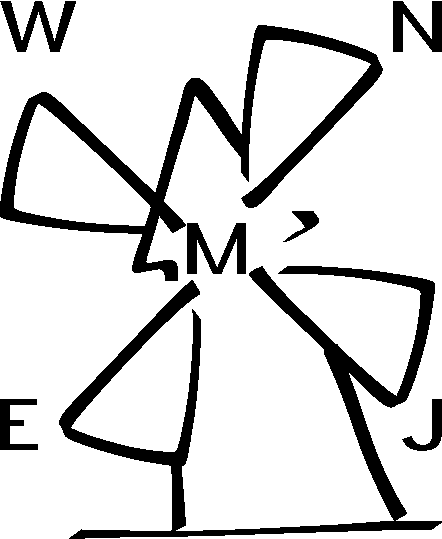
\includegraphics[width=1cm]{ nwejm-logo-NB }
}
\hbox_set_to_wd:Nnn \l__nwejm_journal_logo_box { 1cm }
{
  \box_move_down:nn
  {
    \box_ht:N \l__nwejm_journal_logo_box / 2
    -
    \box_ht:N \l__nwejm_journal_name_box / 2
  }
  {
    \box_use:N \l__nwejm_journal_logo_box
  }
}
\box_set_ht:Nn \l__nwejm_journal_logo_box { \c_zero_dim }
\box_set_dp:Nn \l__nwejm_journal_logo_box { \c_zero_dim }
}
\newpagestyle{__nwejm_article_title_ps}[]{%
  % \widenhead{\c_zero_dim}{\c_zero_dim}
  \sethead%
  {
    \box_use:N \l__nwejm_journal_name_box
  }%
  {%
  }%
  {
    \box_use:N \l__nwejm_journal_logo_box
  }%
  %
  \setfoot%
  {}%
  {\thepage}%
  {}%
}
\def\@pnumwidth{\@tocrmarg}
\AtBeginDocument{%
  \graphicspath{{\c__nwejm_issue_images_path_string_tl//}{../\c__nwejm_issue_images_path_string_tl//}}
  % \glsdisablehyper
}
    \AtBeginDocument{\g__nwejm_mainmatter_switch_tl}
\int_new:N \g__nwejm_issue_number_int
\int_new:N \g__nwejm_issue_month_int
\int_new:N \g__nwejm_issue_year_int
\tl_new:N \g__nwejm_frontcover_image_options_tl
\keys_define:nn { nwejm/issuesetup }
{
  number .int_gset:N = \g__nwejm_issue_number_int,
  volume .int_gset:N = \g__nwejm_issue_volume_int,
  volume .value_required:n = true,
  volume .initial:n = 0,
}
\keys_define:nn { nwejm/dates }
{
  received   .code:n = {
    \tl_gset:Nn \g__nwejm_reception_date_tl {#1}
    \bool_gset_true:N \g__nwejm_date_specified_bool
  },
  accepted   .code:n = {
    \tl_gset:Nn \g__nwejm_acception_date_tl {#1}
    \bool_gset_true:N \g__nwejm_date_specified_bool
  },
  online   .code:n = {
    \tl_gset:Nn \g__nwejm_online_date_tl {#1}
    \bool_gset_true:N \g__nwejm_date_specified_bool
  },
  received .value_required:n = true,
  accepted .value_required:n = true,
  online   .value_required:n = true,
}
\quark_new:N \q__nwejm
\int_new:N \l_author_int
\prop_new:N \g_authors_prop
\prop_new:N \l_affiliations_tagged_prop
\cs_generate_variant:Nn \prop_put_if_new:Nnn { NVn }
\cs_generate_variant:Nn \prop_gput_if_new:Nnn { Nxn }
\cs_generate_variant:Nn \prop_put_if_new:Nnn { NnV }
\cs_new:Npn \__nwejm_prop_count:nn #1#2 { + 1 }
\cs_new:Npn \__nwejm_prop_count:N #1
{ \int_eval:n { 0 \prop_map_function:NN #1 \__nwejm_prop_count:nn } }
\NewDocumentCommand \__nwejm_author_affiliation:ww { o u\q__nwejm }
{
  \stepcounter{footnote}
  \prop_put_if_new:NVn \l_tmpa_prop {\the\c@footnote} {#2}
  \IfValueT{#1}{%
    \prop_put_if_new:NnV \l_affiliations_tagged_prop {#1} {\the\c@footnote}
  }
}
\keys_define:nn { nwejm / authors }
{
  email .tl_gset:N = \g__nwejm_people_email_tl,
  affiliation .code:n = {%
    \__nwejm_author_affiliation:ww #1 \q__nwejm
  },
  affiliationtagged .code:n = {%
    \prop_get:NnNTF \l_affiliations_tagged_prop {#1} \l_tmpa_tl
    {%
      \prop_put_if_new:NVn \l_tmpa_prop {\l_tmpa_tl} {}
    }{
      \msg_error:nnn{__nwejm}{Unknown~tag}{#1}
    }
  },
  affiliation .value_required:n = true,
  affiliationtagged .value_required:n = true,
}
\tl_new:N \l__nwejm_newtheorem_style_tl
\keys_define:nn { nwejm / newtheorem }
{
  title .tl_set:N = \l__nwejm_newtheorem_title_tl,
  title / french .tl_set:N = \l__nwejm_newtheorem_french_title_tl,
  title / english .tl_set:N = \l__nwejm_newtheorem_english_title_tl,
  title / german .tl_set:N = \l__nwejm_newtheorem_german_title_tl,
  title / dutch .tl_set:N = \l__nwejm_newtheorem_dutch_title_tl,
  title .value_required:n = true,
  title / french .value_required:n = true,
  title / english .value_required:n = true,
  title / german .value_required:n = true,
  title / dutch .value_required:n = true,
  %
  style .choice:,
  style / theorem .code:n = {\__nwejm_theorem_style:n {theorem}},
  style / definition .code:n = {\__nwejm_theorem_style:n {definition}},
  style / proof .code:n = {\__nwejm_theorem_style:n {proof}},
  style / unknown .code:n =
  \msg_error:nnxxx { nwejm } { Unknown~choice }
  { style } % Name of choice key
  { theorem~or~definition~or~proof } % Valid choices
  { \exp_not:n {#1} } % Invalid choice given
}
\bool_new:N \g__nwejm_gradient_nabla_bool
\bool_new:N \g__nwejm_gradient_nabla_control_bool
\keys_define:nn { nwejm/articlesetup }
{
  gradient .choice:,
  gradient / nabla .code:n = {\bool_gset_true:N \g__nwejm_gradient_nabla_bool},
  gradient / grad .code:n = {\bool_gset_false:N \g__nwejm_gradient_nabla_bool},
  gradient / unknown .code:n =
  \msg_error:nnxxx { nwejmart } { Unknown~choice }
  { gradient } % Name of choice key
  { nabla~or~grad } % Valid choices
  { \exp_not:n {#1} } % Invalid choice given
}
\tl_new:N \g__nwejm_nwejm_short_string_tl
\tl_new:N \g__nwejm_nwejm_string_tl
\tl_gset:Nn \g__nwejm_nwejm_short_string_tl {
  \cs_if_exist:cTF {texorpdfstring}
  {
    \texorpdfstring{\emph{\c__nwejm_journal_short_title_string_tl}}{\c__nwejm_journal_short_title_string_tl}
  }{%
    \emph{\c__nwejm_journal_short_title_string_tl}
  }%
}
\tl_gset:Nn \g__nwejm_nwejm_string_tl {
  \cs_if_exist:cTF {texorpdfstring}
  {
    \texorpdfstring{\emph{\c__nwejm_journal_title_string_tl}}{\c__nwejm_journal_title_string_tl}
  }{%
    \emph{\c__nwejm_journal_title_string_tl}
  }%
}
\cs_new_protected:Nn \__nwejm_email:n
  {
    \href{mailto:#1}{\nolinkurl{#1}}%
  }
\tl_new:N \l__nwejm_crossref_tl
\cs_new_protected:Nn \__nwejm_populate_bib_file:nn
{
  \int_if_exist:cF {g__nwejm_#2_int}
  {
    \int_new:c {g__nwejm_#2_int}
  }
  \int_incr:c {g__nwejm_#2_int}
  \tl_if_in:nnTF { #2 } { author } {
    \tl_set:Nn \l__nwejm_crossref_tl {%
      \c__nwejm_issue_bib_key_tl
      -art-
      \int_use:N \g__nwejm_articles_int
    }
  } {
    \tl_set:Nn \l__nwejm_crossref_tl {\c__nwejm_issue_bib_key_tl}
  }
  \tl_set:Nn \l__nwejm_people_first_last_name_tl {#1}
  \iow_now:Nx \g__nwejm_bib_out_iow {%
    @article{
      \c__nwejm_issue_bib_key_tl -#2- \int_use:c {g__nwejm_#2_int},
      \iow_newline:
      author={\exp_not:V\l__nwejm_people_first_last_name_tl},
      \iow_newline:
      options={skipbib},
      \iow_newline:
      crossref  = {\l__nwejm_crossref_tl}
      \iow_newline:
    }
    \iow_newline:
  }%
}
\cs_new_protected:Nn \__nwejm_date:nn
{
  \tl_if_exist:NT {#2}
  {
    \tl_if_empty:NF {#2}
    {
      \tl_if_eq:NNF {\c__nwejm_date_received_tl} {#1} { \c__nwejm_dates_separator_tl }
      \tl_mixed_case:n { \exp_args:No \GetTranslation{#1} }
      \c__nwejm_colon_tl\c_space_tl
      \DTMdate{#2}%
    }
  }
}
\tl_new:N \g__nwejm_display_dates_tl%
\tl_gset:Nn \g__nwejm_display_dates_tl {%
  \footnotesize%
  \__nwejm_date:nn {\c__nwejm_date_received_tl}{\g__nwejm_reception_date_tl}
  \__nwejm_date:nn {\c__nwejm_date_accepted_tl}{\g__nwejm_acception_date_tl}
  \__nwejm_date:nn {\c__nwejm_date_online_tl}  {\g__nwejm_online_date_tl}
  \tl_gclear:N \g__nwejm_reception_date_tl
  \tl_gclear:N \g__nwejm_acception_date_tl
  \tl_gclear:N \g__nwejm_online_date_tl
}
\tl_new:N \g__nwejm_keywords_tl
\NewDocumentCommand \keywords { O{} m } {
  \tl_gclear:N \g__nwejm_keywords_tl
  \tl_clear:N \l_tmpb_clist
  \clist_set:Nn \l_tmpb_clist {#2}
  \tl_set:Nx \g__nwejm_keywords_tl { \clist_use:Nnnn \l_tmpb_clist { ,~ } { ,~ } { ,~ } }
  \tl_if_empty:nTF {#1} {%
    \hypersetup{pdfkeywords={\g__nwejm_keywords_tl}}
  }{
    \clist_set:Nn \l_tmpb_clist {#1}
    \hypersetup{pdfkeywords={\clist_use:Nnnn \l_tmpb_clist { ,~ } { ,~ } { ,~ }}}
  }
}
\tl_new:N \g__nwejm_msc_tl
\NewDocumentCommand \msc { m } {
  \tl_gclear:N \g__nwejm_msc_tl
  \tl_clear:N \l_tmpa_clist
  \clist_set:Nn \l_tmpa_clist {#1}
  \tl_set:Nn \g__nwejm_msc_tl { \clist_use:Nnnn \l_tmpa_clist { ,~ } { ,~ } { ,~ } }
%%<class-article>    \hypersetup{pdfmsc=\g_@@_msc_tl}
}

\file_if_exist:nT { \c__nwejm_main_file_name_tl.aux }
{\externaldocument[__nwejm-]{\c__nwejm_main_file_name_tl}
  \AtBeginDocument{\setcounter{page}{\number\numexpr\getpagerefnumber{__nwejm-\currfilebase}}}
}
\vref@addto\extrasfrench{%
  \def\reftextfaceafter {page~\reftextvario{ci-contre}{suivante}}%
  \def\reftextfacebefore{page~\reftextvario{ci-contre}%
    {pr\'ec\'edente}}%
  \def\reftextafter
  {page~suivante}%
  \def\reftextbefore
  {page~pr\'ec\'edente}%
  \def\reftextcurrent {de~la~pr\'esente~page}%
  \def\reftextfaraway#1{p.\nobreakspace\pageref{#1}}%
  \def\reftextpagerange#1#2{p.\nobreakspace\pageref{#1}--\pageref{#2}}%
  \def\reftextlabelrange#1#2{\ref{#1}~\‘a\nobreakspace\ref{#2}}%
}
\vref@addto\extrasngerman{%
  \def\reftextfaceafter {auf~der~n\"achsten~Seite}%
  \def\reftextfacebefore{auf~der~vorherigen~Seite}%
  \let\reftextafter     \reftextfaceafter
  \let\reftextbefore    \reftextfacebefore
  \def\reftextcurrent   {auf~dieser~Seite}%
  \def\reftextfaraway#1{auf~S.\nobreakspace\pageref{#1}}%
  \def\reftextpagerange#1#2{auf~den~S.\nobreakspace\pageref{#1}--\pageref{#2}}%
  \def\reftextlabelrange#1#2{\ref{#1}~bis\nobreakspace\ref{#2}}%
}
\vref@addto\extrasdutch{%
  \def\refpagename{pagina}%
  \def\reftextfaceafter {op~de~\reftextvario{rechter~\refpagename}%
    {\refpagename\ hiernaast}}%
  \def\reftextfacebefore{op~de~\reftextvario{linker~\refpagename}%
    {\refpagename\ hiernaast}}%
  \def\reftextafter     {op~de~\reftextvario{volgende~\refpagename}%
    {\refpagename\ hierna}}%
  \def\reftextbefore    {op~de~\reftextvario{vorige~\refpagename}%
    {\refpagename\ hiervoor}}%
  \def\reftextcurrent   {op~deze~\refpagename}%
  \def\reftextfaraway#1{op~\refpagename\nobreakspace\pageref{#1}}
}
\vref@addto\extrasenglish{%
  \def\reftextfaceafter {on~the~\reftextvario{facing}{next}~page}%
  \def\reftextfacebefore{on~the~\reftextvario{facing}{preceding}~page}%
  \def\reftextafter     {on~the~\reftextvario{following}{next}~page}%
  \def\reftextbefore    {on~the~\reftextvario{preceding}{previous}~page}%
  \def\reftextcurrent   {on~\reftextvario{this}{the~current}~page}%
  \def\reftextfaraway#1{on~p.\nobreakspace\pageref{#1}}%
  \def\reftextpagerange#1#2{on~pp.\nobreakspace\pageref{#1}--\pageref{#2}}%
  \def\reftextlabelrange#1#2{\ref{#1}~to\nobreakspace\ref{#2}}%
}
\def\reftextvario#1#2{#2}
\cs_new_protected:Nn \__nwejm_command_only_in_body:n
{
  \cs_if_eq:NNF {\@onlypreamble} {\@notprerr} {
    \msg_error:nnn{
     nwejmart
     }{Command~restricted~to~document~body~used~in~preamble}{#1}
  }
}
\NewDocumentCommand \articlesetup { m } {
  \__nwejm_command_only_in_body:n {\articlesetup}
  \keys_set:nn { nwejm/articlesetup } {#1}
}
\NewDocumentCommand \dates { m } {
  \keys_set:nn { nwejm/dates } { #1 }
}
\tl_gset:Nn \g__nwejm_french_crefname_tl {
  \clist_set:Nn \l_tmpa_clist {%
    theorem,
    corollary,
    conjecture,
    proposition,
    lemma,
    axiom,
    definition,
    remark,
    example,
    notation,
    proof%
  }
  \clist_map_inline:Nn \l_tmpa_clist {
    \crefname{#1}{
      \tl_lower_case:n{
        \GetTranslationFor{french}{#1}
      }
    }{%
      \tl_lower_case:n{
        \GetTranslationFor{french}{plural-#1}
      }
    }
  }
  \crefname{equation}{{\'e}quation}{{\'e}quations}%
  \crefname{figure}{figure}{figures}%
  \crefname{table}{table}{tables}%
  \crefname{page}{page}{pages}%
  \crefname{part}{partie}{parties}%
  \crefname{chapter}{chapitre}{chapitres}%
  \crefname{section}{section}{sections}%
  \crefname{appendix}{annexe}{annexes}%
  \crefname{enumi}{point}{points}%
  \crefname{footnote}{note}{notes}%
  \crefname{theorem}{th\'eor\`eme}{th\'eor\`emes}%
  \crefname{lemma}{lemme}{lemmes}%
  \crefname{corollary}{corollaire}{corollaires}%
  \crefname{proposition}{proposition}{propositions}%
  \crefname{definition}{d\'efinition}{d\'efinitions}%
  \crefname{result}{r\'esultat}{r\'esultats}%
  \crefname{example}{exemple}{exemples}%
  \crefname{remark}{remarque}{remarques}%
  \crefname{note}{commentaire}{commentaires}%
  \crefname{algorithm}{algorithme}{algorithmes}%
  \crefname{listing}{liste}{listes}%
  \crefname{line}{ligne}{lignes}%
}
\NewDocumentCommand \inputarticle { O{english} m } {%
  \newrefsection
  \tl_if_eq:nnTF { #1 } { german } {%
    \selectlanguage{ngerman}
  }{
    \tl_if_eq:nnTF { #1 } { french } {%
      \selectlanguage{french}
      \g__nwejm_french_crefname_tl
    }{
      \selectlanguage{#1}
    }
  }%
  \tl_if_eq:nnTF { #1 } { french } {%
    \FrenchFootnotes
  }{%
    \StandardFootnotes
  }
  \inputfrom{./}{#2}
  \clist_put_right:Nn \g__nwejm_counters_to_be_reset_clist {
    footnote,
    section,
    figure,
    table,
    equation
  }
  \clist_map_inline:Nn \g__nwejm_counters_to_be_reset_clist {
    \@ifundefined{c@##1}{
    }{
      \setcounter{##1}{\c_zero}
    }
  }
  \glsresetall
  \selectlanguage{english}
}
\AtBeginDocument{%
\tl_new:N \g__nwejm_bib_issue_date_tl
\tl_gset:Nn
\g__nwejm_bib_issue_date_tl {
  \int_use:N \g__nwejm_issue_year_int -
  \int_compare:nNnT {\g__nwejm_issue_month_int}<{10}
  {
    0
  }
  \int_use:N \g__nwejm_issue_month_int
}
  \iow_now:Nx \g__nwejm_bib_out_iow {%
    @periodical{\c__nwejm_issue_bib_key_tl,\iow_newline:
      issuetitle   = {\exp_not:f\c__nwejm_journal_title_string_tl},\iow_newline:
      date         = {\g__nwejm_bib_issue_date_tl},\iow_newline:
      number       = \int_use:N \g__nwejm_issue_number_int,\iow_newline:
      % issn         = {\l__nwejm_journal_issn_tl},\iow_newline:
      options      = {skipbib}\iow_newline:
    }
    \iow_newline:
  }%
}
\tl_new:N \g__nwejm_title_tl
\RenewDocumentCommand \title { o o m } {
  \cleardoublepage
  \int_gincr:N \g__nwejm_articles_int
  \tl_gclear:N \g__nwejm_short_title_tl
  \tl_gclear:N \g__nwejm_header_title_tl
  \tl_gclear:N \g__nwejm_short_subtitle_tl
  %
  \IfNoValueF {#1}
  {
    \tl_gset:Nn \g__nwejm_short_title_tl {#1}
  }
  \IfNoValueF {#2}
  {
    \tl_gset:Nn \g__nwejm_header_title_tl {#2}
  }
  \tl_gset:Nn \g__nwejm_title_tl {#3}
  \tl_if_empty:NT \g__nwejm_short_title_tl {%
    \tl_gset_eq:NN \g__nwejm_short_title_tl \g__nwejm_title_tl
  }
  \tl_if_empty:NT \g__nwejm_header_title_tl {%
    \tl_gset_eq:NN \g__nwejm_header_title_tl \g__nwejm_short_title_tl
  }
}
\tl_new:N \g__nwejm_subtitle_tl
\NewDocumentCommand \subtitle { o m } {
  \IfNoValueF {#1}
  {
    \tl_gset:Nn \g__nwejm_short_subtitle_tl {#1}
  }
  \tl_gset:Nn \g__nwejm_subtitle_tl {#2}
  \tl_if_empty:NT \g__nwejm_short_subtitle_tl {%
    \tl_gset_eq:NN \g__nwejm_short_subtitle_tl \g__nwejm_subtitle_tl
  }
}
\RenewDocumentCommand \author { O{} m } {
  \cleardoublepage
  \int_incr:N \l_author_int
  \prop_gput_if_new:Nxn \g_authors_prop {author_\int_use:c {l_author_int}} {#2}
  \IfNoValueF {#1}
  {
    \keys_set:nn { nwejm/authors } { #1 }
  }
  \prop_set_eq:cN {l_author_ \int_use:c {l_author_int} _affiliations_prop} \l_tmpa_prop
  \prop_clear:N \l_tmpa_prop
  \__nwejm_populate_bib_file:nn {#2}{author-art-\int_use:N \g__nwejm_articles_int}
  \tl_if_empty:NTF \l__nwejm_people_first_last_names_tl {%
    \tl_put_right:Nn
    \l__nwejm_people_first_last_names_tl
    {#2}
  }{
    \tl_put_right:Nn
    \l__nwejm_people_first_last_names_tl
    {~and~#2}
  }
}
\iow_new:N \g__nwejm_bib_out_iow
\ior_new:N \g__nwejm_bib_out_ior
\tl_new:N \g__nwejm_bib_out_tl
\file_if_exist:nTF { \c__nwejm_issue_bib_path_string_tl }
{
  \ior_open:Nn \g__nwejm_bib_out_ior { \c__nwejm_issue_bib_path_string_tl }
  \ior_str_map_inline:Nn \g__nwejm_bib_out_ior
  { \tl_gput_right:Nn \g__nwejm_bib_out_tl {#1 \par } }
  \ior_close:N \g__nwejm_bib_out_ior
}{
  \typeout{no file! rerun}
}
\iow_open:Nn \g__nwejm_bib_out_iow { \c__nwejm_issue_bib_path_string_tl }
\tl_new:N \g__nwejm_abstract_body_tl
\NewDocumentEnvironment{abstract}{}
  {\CollectAbstract}
  {\endCollectAbstract}
\NewEnviron{CollectAbstract}
  {
    \tl_gset_eq:NN \g__nwejm_abstract_body_tl \BODY
  }
\tl_new:N \g__nwejm_frontmatter_switch_tl%
\tl_gset:Nn \g__nwejm_frontmatter_switch_tl {
  \bool_gset_true:N  \g__nwejm_frontmatter_bool
  \frontmatter
  \pagestyle{__nwejm_frontmatter_ps}%
  \exp_after:wN\newgeometry\exp_after:wN{\c__nwejm_main_geometry_tl}%
}
\tl_new:N \g__nwejm_mainmatter_switch_tl%
\tl_gset:Nn \g__nwejm_mainmatter_switch_tl {
  \bool_gset_false:N \g__nwejm_frontmatter_bool
  \bool_gset_true:N \g__nwejm_mainmatter_bool
  \mainmatter
  % \SetParskip{\c__nwejm_mainmatter_parskip_skip}
  \pagestyle{__nwejm_mainmatter_ps}%
  \exp_after:wN\newgeometry\exp_after:wN{\c__nwejm_main_geometry_tl}%
}
\tl_new:N \g__nwejm_article_acknowledgments_tl%
\cs_new_protected:Nn \__nwejm_article_acknowledgments:n
{
  \tl_gset:Nn \g__nwejm_article_acknowledgments_tl { #1 }
}
\NewDocumentCommand \acknowledgments { m } {
  \__nwejm_article_acknowledgments:n {#1}
}
\tl_new:N \g__nwejm_article_bib_key_tl%
\tl_new:N \l__nwejm_people_first_last_names_tl
\tl_new:N \g__nwejm_authors_first_last_names_tl%
\tl_new:N \g__nwejm_citeauthor_no_giveninits%
\tl_new:N \g__nwejm_citeauthor_tl%
\int_new:N \g__nwejm_author_s_number_current_article_int%
\cs_new_protected:Nn \__nwejm_citeauthor_no_giveninits:n {%
  \tl_gset:Nn \g__nwejm_citeauthor_tl {%
    \DeclareNameAlias{labelname}{default}%
    \group_begin:
    \togglefalse{abx@bool@giveninits}%
    \citeauthor{#1}
    \group_end:
  }%
  \cs_if_exist:cTF {texorpdfstring}
  {
    \texorpdfstring{\g__nwejm_citeauthor_tl}{}
  }{%
    \g__nwejm_citeauthor_tl
  }%
}
\cs_set_eq:NN \__nwejm_orig_multinamedelim \multinamedelim
\cs_set_eq:NN \__nwejm_orig_finalnamedelim \finalnamedelim
\cs_new_protected:Nn \__nwejm_maketitle_citeauthor:n
{
  \restorecommand\mkbibnamelast
  \def\multinamedelim  {\hskip 1em \@plus.17fil}%
  \cs_set_eq:NN \finalnamedelim \multinamedelim
  \AtNextCitekey{\defcounter{maxnames}{100}}
  \group_begin:
  \DeclareNameAlias{labelname}{default}%
  \togglefalse{abx@bool@giveninits}%
  \citeauthor{#1}
  \group_end:
  \cs_set_eq:NN \multinamedelim \__nwejm_orig_multinamedelim
  \cs_set_eq:NN \finalnamedelim \__nwejm_orig_finalnamedelim
  \protected\def\mkbibnamelast#1{%
    \textsc{\textnohyphenation{#1}}}%
}
\cs_new_protected:Nn \__nwejm_display_author:n
{
  \seq_clear:N \l_tmpa_seq
  \prop_get:NnN \g_authors_prop {author_#1} \l_tmpa_tl
  \prop_map_inline:cn {l_author_ #1 _affiliations_prop} {
    \seq_put_right:Nx \l_tmpa_seq { ##1 }
  }
  \seq_sort:Nn \l_tmpa_seq
  {
    \int_compare:nNnTF { ##1 } > { ##2 }
    { \sort_return_swapped: }
    { \sort_return_same: }
  }
  \mbox{%
    \__nwejm_citeauthor_no_giveninits:n {\c__nwejm_issue_bib_key_tl -author-art- \int_use:N \g__nwejm_articles_int-#1}
  }
  \seq_map_inline:Nn \l_tmpa_seq {
    \prop_get:cnN {l_author_ #1 _affiliations_prop} {##1} \l_tmpb_tl
    \footnotemark[##1]
    \tl_if_empty:NF \l_tmpb_tl
    {
      \footnotetext[##1]{\l_tmpb_tl}
    }
  }
  \hskip 1em plus .17fil
}
\tl_new:N \l__nwejm_bullet_and_rule_tl
\tl_new:N \l__nwejm_authors_box_tl
\tl_new:N \l__nwejm_abstract_box_tl
\tl_new:N \l__nwejm_bullet_and_rule_odd_tl
\tl_new:N \l__nwejm_bullet_and_rule_even_tl
\tl_new:N \l__nwejm_title_box_tl
\tl_new:N \g__nwejm_title_for_toc_tl
\RenewDocumentCommand \maketitle { } {
\tl_gset:Nn \g__nwejm_article_bib_key_tl {%
  \c__nwejm_issue_bib_key_tl
  -art-
  \int_use:N \g__nwejm_articles_int
}
\tl_if_empty:NF \g__nwejm_title_tl {%
  \iow_now:Nx \g__nwejm_bib_out_iow {%
    @article{
      \g__nwejm_article_bib_key_tl,
      \iow_newline:
      title={\exp_not:V\g__nwejm_title_tl},
      \iow_newline:
      \tl_if_empty:NF \g__nwejm_subtitle_tl {%
        subtitle={\exp_not:V\g__nwejm_subtitle_tl},
        \iow_newline:
      }
      \tl_if_eq:NNF { \g__nwejm_short_title_tl } { \g__nwejm_title_tl } {%
        shorttitle={\exp_not:V\g__nwejm_short_title_tl},
        \iow_newline:
      }%
      \tl_if_empty:NF \l__nwejm_people_first_last_names_tl
      {
        author={\exp_not:V\l__nwejm_people_first_last_names_tl},
        \iow_newline:
      }
      options={skipbib},
      \iow_newline:
      crossref  = {\c__nwejm_issue_bib_key_tl}
    }
    \iow_newline:
  }%
  % \tl_clear:N \l__nwejm_people_first_last_names_tl
}%
\tl_set:Nn \l__nwejm_authors_box_tl
{%
  \bool_if:nTF { \tl_if_empty_p:N \l__nwejm_people_first_last_names_tl }
  {
    \mbox{}
  }
  {
    \int_set:Nn \l_tmpa_int { \__nwejm_prop_count:N \g_authors_prop}
    \normalsize%
    \int_step_inline:nnnn {1}{1}{\l_tmpa_int} {
      \__nwejm_display_author:n {##1}
    }
    \prop_gclear:N \g_authors_prop
  }
}
\int_zero:N \l_author_int
\prop_clear:N \l_affiliations_tagged_prop
\tl_set:Nn \l__nwejm_dates_box_tl
{%
  \g__nwejm_display_dates_tl
}
\tl_set:Nn \l__nwejm_keywords_box_tl
{%
  \noindent
  {
    \bfseries
    \tl_mixed_case:n{
      \GetTranslation{plural-keyword}
      \c__nwejm_colon_tl
    }
  }
  \c_space_tl\g__nwejm_keywords_tl.
}
\tl_set:Nn \l__nwejm_msc_box_tl
{%
  \noindent\textbf{\c__nwejm_msc_string_tl}\c__nwejm_colon_tl\c_space_tl\g__nwejm_msc_tl.
}
\tl_set:Nn \l__nwejm_abstract_box_tl
{%
  \mbox{}
  \par%
  \vskip .5em%
  \tl_if_empty:NTF \g__nwejm_abstract_body_tl
  {%
    \msg_warning:nn{nwejmart}{No~abstract}
  }%
  {%
    \small
    \begin{center}%
      {\bfseries \abstractname\vspace{-.5em}\vspace{\z@}}%
    \end{center}%
    \begin{quotation}
      \g__nwejm_abstract_body_tl
    \end{quotation}
  }
}%
\tl_set:Nn \g__nwejm_partial_title_for_toc_tl
{
  \tl_if_empty:NTF \g__nwejm_short_title_tl {%
    \g__nwejm_title_tl%
  }{
    \g__nwejm_short_title_tl%
  }
  \bool_if:nF { \tl_if_empty_p:N \g__nwejm_short_subtitle_tl }
  {
    .\c_space_tl\g__nwejm_short_subtitle_tl
  }
}
    \hypersetup{pdftitle=\g__nwejm_partial_title_for_toc_tl}
\tl_set:Nn \g__nwejm_title_for_toc_tl
{
  \g__nwejm_partial_title_for_toc_tl
  \bool_if:nF { \tl_if_empty_p:N \l__nwejm_people_first_last_names_tl }
  {
    \textsl{
      \cs_if_exist:cTF {texorpdfstring}
      {
        \texorpdfstring{%
          \AtNextCitekey{\defcounter{maxnames}{100}}
          \c_space_tl\textendash\c_space_tl\citeauthor{\g__nwejm_article_bib_key_tl}
        }{}
      }{%
        \c_space_tl\textendash\c_space_tl\citeauthor{\g__nwejm_article_bib_key_tl}
      }%
    }
  }
}
  \setsecnumdepth{none}
 \bookmarksetup{depth=-2}
  \chapter[\g__nwejm_title_for_toc_tl]{%
    \LARGE%
    \g__nwejm_title_tl
    \tl_if_empty:NF \g__nwejm_subtitle_tl {%
      \\[1ex]%
      \Large%
      \g__nwejm_subtitle_tl
    }\\[2ex]%
    \l__nwejm_authors_box_tl%
    \bool_if:NT {\g__nwejm_date_specified_bool}
    {
      \\[2ex]
      \l__nwejm_dates_box_tl
    }
    \\[-4ex]
  }
\label{\currfilebase}
  \bool_gset_false:N \g__nwejm_date_specified_bool
  \bookmarksetup{depth=subsection}
  \setsecnumdepth{subsection}
  \thispagestyle{__nwejm_article_title_ps}%
\l__nwejm_abstract_box_tl%
\normalsize
\tl_if_empty:NTF \g__nwejm_keywords_tl {
  \msg_warning:nn{nwejmart}{No~keyword}
}{
  \l__nwejm_keywords_box_tl
  \par%
  \vskip .5em%
}
\tl_if_empty:NTF \g__nwejm_msc_tl {
  \msg_warning:nn{nwejmart}{No~MSC}
}{
  \l__nwejm_msc_box_tl
  \par%
  \vskip .5em%
}
 \hypersetup{pdfauthor=\l__nwejm_people_first_last_names_tl}
\tl_gclear:N \g__nwejm_title_tl
\tl_gclear:N \g__nwejm_subtitle_tl
\tl_gclear:N \g__nwejm_title_for_toc_tl
\tl_gclear:N \g__nwejm_abstract_body_tl
  \tl_gclear:N \g__nwejm_people_affiliation_tl
  \tl_gclear:N \g__nwejm_people_email_tl
  \tl_clear:N \l__nwejm_people_first_last_names_tl%
}
\DeclarePlainStyle{«~}{~»}{`}{'}
\setcounter{topnumber}{3}
\renewcommand{\topfraction}{0.8}
\addtolength{\skip\footins}{.25\baselineskip}
\setlength{\columnsep}{7mm}%
\renewcommand{\thesection}{\arabic{section}}%
\@ifpackageloaded{siunitx}{%
  \addto\extrasenglish{\sisetup{locale = UK}}
  \addto\extrasfrench{\sisetup{locale = FR}}
  \addto\extrasngerman{\sisetup{locale = DE}}
  \addto\extrasgerman{\sisetup{locale = DE}}
  \addto\extrasdutch{%
    \sisetup{%
      exponent-product      = \ensuremath { \times } ,
      inter-unit-product    = \,                     ,
      output-decimal-marker = { , }
    }%
  }
  \sisetup{detect-all}
}
\apptocmd{\appendix}{\renewcommand{\thesection}{\Alph{section}}}{}{}
\cs_set_eq:NN \__nwejm_section \section
\cs_set_eq:NN \__nwejm_subsection \subsection
\cs_set_eq:NN \__nwejm_subsubsection \subsubsection
\AfterPreamble{%
  \RenewDocumentCommand \section { s o o m } {%
    \tl_gclear:N \g__nwejm_short_section_title_tl
    \IfBooleanTF {#1}
    {
      \setsecnumdepth{none}%
    }
    {
      \resetsecnumdepth*%
    }
    \tl_gset:Nn \g__nwejm_section_title_tl {#4}
    \IfNoValueTF{#2}{
      \tl_gset:Nn \g__nwejm_short_section_title_tl {#4}
    }{
      \tl_gset:Nn \g__nwejm_short_section_title_tl {#2}
    }
    \__nwejm_section[\g__nwejm_short_section_title_tl]{\g__nwejm_section_title_tl}
    \IfNoValueF {#3}{
      \sectionmark{#3}
    }
  }
  \RenewDocumentCommand \subsection { s o m } {%
    \IfBooleanT {#1}
    {
      \setsecnumdepth{none}%
    }
    \IfNoValueTF{#2}{\__nwejm_subsection{#3}}{\__nwejm_subsection[#2]{#3}}
  }
  \RenewDocumentCommand \subsubsection { s o m } {%
    \IfBooleanT {#1}
    {
      \setsecnumdepth{none}%
    }
    \IfNoValueTF{#2}{\__nwejm_subsubsection{#3}}{\__nwejm_subsubsection[#2]{#3}}
  }
}
\int_new:N \l__nwejm_abs_int
\cs_new_protected:Nn \__nwejm_ordinalnum_suffix:n
{
  \int_set:Nn \l__nwejm_abs_int {\int_abs:n {#1}}
  \ifcurrentbaselanguage{english}{
    \int_use:N \l__nwejm_abs_int
    \int_set:Nn \l_tmpa_int {\int_mod:nn {\l__nwejm_abs_int} {\c_one_hundred}}
    \int_case:nnF
    { \l_tmpa_int }
    {
      { \c_eleven }   { \fmtord{th} }
      { \c_twelve }   { \fmtord{th} }
      { \c_thirteen } { \fmtord{th} }
    }{
      \int_set:Nn \l_tmpb_int {\int_mod:nn {\l__nwejm_abs_int} {\c_ten}}
      \int_case:nnF
      { \l_tmpb_int }
      {
        { \c_zero }   { \fmtord{th} }
        { \c_one }   { \fmtord{st} }
        { \c_two }   { \fmtord{nd} }
        { \c_three } { \fmtord{rd} }
      }{
        \fmtord{th}
      }
    }
  }{
    \ifcurrentbaselanguage{dutch}{
      \int_use:N \l__nwejm_abs_int
      e
    }{
      \textsc{\int_to_roman:n {\int_abs:n {#1}}}
      \ifcurrentbaselanguage{french}{
        \int_compare:nNnTF { \l__nwejm_abs_int } = { 1 }{\fmtord{er}}{\fmtord{e}}
      }{
        \ifcurrentbaselanguage{german}{
          .
        }{
          \ifcurrentbaselanguage{ngerman}{
            .
          }{
          }
        }
      }
    }
  }
}
\cs_new_protected:Nn \__nwejm_century_suffix:n
{
  \c_space_tl{}
  \GetTranslation{century}%
  \int_compare:nNnT { #1 } < { 0 }{
    \c_space_tl
    \GetTranslation{before-christ}
  }{
  }
}
\DeclareCaptionLabelSeparator{dash}{\nobreakspace--\nobreakspace}
\captionsetup{
   labelsep=dash
 }
\NewDocumentCommand \century { s m } {%
  \__nwejm_ordinalnum_suffix:n {#2}%
  \IfBooleanTF {#1}
  {
    \int_compare:nNnT { #2 } < { 0 }{
      \__nwejm_century_suffix:n {#2}%
    }
  }{
    \__nwejm_century_suffix:n {#2}%
  }
  \int_compare:nNnT { #2 } < { 0 }{
    \ifcurrentbaselanguage{english}{%
    }{
      \@ifnextchar.%
      {
      }{
        .\xspace
      }%
    }
  }
}
\NewDocumentCommand \aside { s m } {%
  \IfBooleanTF {#1}
  {
    \c__nwejm_aside_string_tl{}~#2
  }
  {
    \c__nwejm_aside_string_tl{}~#2~\c__nwejm_aside_string_tl
  }
}
\NewDocumentCommand \ie { s } {%
  \IfBooleanTF {#1}
  {
    \GetTranslation{idest}
  }
  {
    \GetTranslation{ie}
    \@ifnextchar.%
    {
    }{
      .\xspace
    }%
  }
}
\NewDocumentCommand \Ie { s } {%
  \IfBooleanTF {#1}
  {
    \GetTranslation{Idest}
  }
  {
    \GetTranslation{Ie}
    \@ifnextchar.%
    {
    }{
      .\xspace
    }%
  }
}
\RenewDocumentCommand \vec { m } {
  \vv{#1}
}
\bool_new:N \g__nwejm_no_numbered_theorem_bool
\cs_new_protected:Nn \__nwejm_theorem_style:n
{
  \bool_gset_false:N \g__nwejm_no_numbered_theorem_bool
  \str_case:nn
  { #1 }
  {
    { theorem }   {
      \theoremstyle{plain}
      \theoremheaderfont{\normalfont\bfseries}
      \theorembodyfont{\itshape}
      \theoremseparator{~--}
      \theoremsymbol{}
    }
    { definition }   {
      \theoremstyle{plain}
      \theoremheaderfont{\normalfont\bfseries}
      \theorembodyfont{\normalfont}
      \theoremseparator{~--}
      \theoremsymbol{}
    }
    { proof }   {
      \theoremstyle{nonumberplain}
      \bool_gset_true:N \g__nwejm_no_numbered_theorem_bool
      \theoremheaderfont{\normalfont\itshape}
      \theorembodyfont{\normalfont}
      \theoremseparator{.}
      \theoremsymbol{\ensuremath{\square}}
    }
  }
}
\cs_set_eq:NN \__nwejm_orig_newtheorem \newtheorem
\cs_new_protected:Nn \__nwejm_new_theorem:nnnnn
{
    \IfTranslation{English}{#1}{%
    }{%
      \DeclareTranslation{English}{#1}{\tl_mixed_case:n{#2}}%
    }
    \IfTranslation{French}{#1}{%
    }{%
      \DeclareTranslation{French}{#1}{\tl_mixed_case:n{#3}}%
    }
    \IfTranslation{German}{#1}{%
    }{%
      \DeclareTranslation{German}{#1}{\tl_mixed_case:n{#4}}%
    }
    \IfTranslation{Dutch}{#1}{%
    }{%
      \DeclareTranslation{Dutch}{#1}{\tl_mixed_case:n{#5}}%
    }
    \__nwejm_orig_newtheorem{#1}{\tl_mixed_case:n{ \GetTranslation{#1} }}
    \bool_if:NF {\g__nwejm_no_numbered_theorem_bool} {
      \__nwejm_orig_newtheorem*{#1__nwejm_nonumbered}{\tl_mixed_case:n{ \GetTranslation{#1} }}
    }
}
\cs_generate_variant:Nn \__nwejm_new_theorem:nnnnn { nVVVV }
\RenewDocumentCommand \newtheorem { O{} m }
{
  \AtBeginDocument{
    \tl_clear:N \l__nwejm_newtheorem_style_tl
    \tl_clear:N \l__nwejm_newtheorem_title_tl
    \tl_clear:N \l__nwejm_newtheorem_french_title_tl
    \tl_clear:N \l__nwejm_newtheorem_english_title_tl
    \tl_clear:N \l__nwejm_newtheorem_german_title_tl
    \tl_clear:N \l__nwejm_newtheorem_dutch_title_tl
    %
    \tl_set:Nn \l__nwejm_newtheorem_english_title_tl {
      #2
    }
    \tl_set:Nf \l__nwejm_newtheorem_french_title_tl {
      \l__nwejm_newtheorem_english_title_tl
    }
    \tl_set:Nf \l__nwejm_newtheorem_german_title_tl {
      \l__nwejm_newtheorem_english_title_tl
    }
    \tl_set:Nf \l__nwejm_newtheorem_dutch_title_tl {
      \l__nwejm_newtheorem_english_title_tl
    }
    \tl_set:Nn \l__nwejm_newtheorem_style_tl {
      theorem
    }
    \__nwejm_theorem_style:n {theorem}
    \IfNoValueF {#1}
    {
      \keys_set:nn { nwejm / newtheorem } { #1 }
      \tl_if_empty:NF \l__nwejm_newtheorem_title_tl {%
        \tl_set:Nf \l__nwejm_newtheorem_english_title_tl
        {
          \l__nwejm_newtheorem_title_tl
        }
        \tl_set:Nf \l__nwejm_newtheorem_french_title_tl
        {
          \l__nwejm_newtheorem_title_tl
        }
        \tl_set:Nf \l__nwejm_newtheorem_german_title_tl
        {
          \l__nwejm_newtheorem_title_tl
        }
        \tl_set:Nf \l__nwejm_newtheorem_dutch_title_tl
        {
          \l__nwejm_newtheorem_title_tl
        }
      }
    }
    %
    \__nwejm_new_theorem:nVVVV
    {#2}
    {\l__nwejm_newtheorem_english_title_tl}
    {\l__nwejm_newtheorem_french_title_tl}
    {\l__nwejm_newtheorem_german_title_tl}
    {\l__nwejm_newtheorem_dutch_title_tl}
    \makesavenoteenv{#2}
    \bool_if:NF {\g__nwejm_no_numbered_theorem_bool} {
      \ifcsmacro{#2*}{%
        \RenewDocumentEnvironment{#2*}{o}
        {
          \IfNoValueTF {##1}
          { \begin{#2__nwejm_nonumbered} }
            { \begin{#2__nwejm_nonumbered}[##1] }
            }{
            \end{#2__nwejm_nonumbered}
          }
        }{
          \NewDocumentEnvironment{#2*}{o}
          {
            \IfNoValueTF {##1}
            { \begin{#2__nwejm_nonumbered} }
              { \begin{#2__nwejm_nonumbered}[##1] }
              }{
              \end{#2__nwejm_nonumbered}
            }
          }
        }
    \clist_put_right:Nn \g__nwejm_counters_to_be_reset_clist {#2}
  }
}
\newtheorem{theorem}
\newtheorem{corollary}
\newtheorem{conjecture}
\newtheorem{proposition}
\newtheorem{lemma}
\newtheorem{axiom}
\newtheorem[style=definition]{definition}
\newtheorem[style=definition]{remark}
\newtheorem[style=definition]{example}
\newtheorem[style=definition]{notation}
\newtheorem[style=proof]{proof}
\cs_new_protected:Nn \__nwejm_clone_theorem:nn
{
  \NewDocumentEnvironment{#1}{}
  {
    \begin{#2}
    }{
    \end{#2}
  }
  \NewDocumentEnvironment{#1*}{}
  {
    \begin{#2*}
    }{
    \end{#2*}
  }
}
\__nwejm_clone_theorem:nn {Theorem}{theorem}
\__nwejm_clone_theorem:nn {Corollary}{corollary}
\__nwejm_clone_theorem:nn {Conjecture}{conjecture}
\__nwejm_clone_theorem:nn {Proposition}{proposition}
\__nwejm_clone_theorem:nn {Lemma}{lemma}
\__nwejm_clone_theorem:nn {Axiom}{axiom}
\__nwejm_clone_theorem:nn {Definition}{definition}
\__nwejm_clone_theorem:nn {Remark}{remark}
\__nwejm_clone_theorem:nn {Example}{example}
\__nwejm_clone_theorem:nn {Notation}{notation}
\__nwejm_clone_theorem:nn {Proof}{proof}
\clist_set:Nn \l_tmpa_clist {%
  theorem,
  corollary,
  conjecture,
  proposition,
  lemma,
  axiom,
  definition,
  remark,
  example,
  notation,
  proof%
}
\clist_map_inline:Nn \l_tmpa_clist {
  \crefname{#1}{
    \tl_mixed_case:n{
      \GetTranslation{#1}
    }
  }{
    \tl_mixed_case:n{
      \GetTranslation{plural-#1}
    }
  }
  \Crefname{#1}{
    \tl_mixed_case:n{
      \GetTranslation{#1}
    }
  }{%
    \tl_mixed_case:n{
      \GetTranslation{plural-#1}
    }
  }
}
\AfterEndPreamble{
  \ifcurrentbaselanguage{french}{\g__nwejm_french_crefname_tl}{}
}
\clist_set:Nn \l_tmpa_clist {%
  hypothesis,
  assertion%
}
\clist_map_inline:Nn \l_tmpa_clist {
  \newlist{#1}{enumerate}{1}
  \setlist[#1]{%
    label=
    \normalfont
    (
    \textsf{
      \tl_upper_case:n {\tl_head:f {\GetTranslation{#1}}}
    }
    $\c_math_subscript_token\mathsf{\arabic*}$),
    ref=(
    \textsf{
      \tl_upper_case:n {\tl_head:f {\GetTranslation{#1}}}
    }
    $_\mathsf{\arabic*}$
    )
  }
  \crefname{#1i}{
    \GetTranslation{#1}
  }{%
    \GetTranslation{plural-#1}
  }
  \Crefname{#1i}{
    \tl_mixed_case:n{
      \GetTranslation{#1}
    }
  }{%
    \tl_mixed_case:n{
      \GetTranslation{plural-#1}
    }
  }
}
\NewDocumentEnvironment{hypotheses}{}
{
  \begin{hypothesis}
  }{
  \end{hypothesis}
}
\NewDocumentEnvironment{assertions}{}
{
  \begin{assertion}
  }{
  \end{assertion}
}
\RenewDocumentCommand{\DeclareMathOperator}{mm}
{
  \NewDocumentCommand{#1}{}
  {
    \operatorname{#2}
    \peek_after:Nw \__nwejm_opx_check:
  }
}
\NewDocumentCommand{\BinaryOperators}{m}
{
  \clist_gput_right:Nn \g__nwejm_opx_binary_clist { #1 }
}
\clist_new:N \g__nwejm_opx_binary_clist
\cs_new_protected:Nn \__nwejm_opx_check:
{
  \clist_map_inline:Nn \g__nwejm_opx_binary_clist
  {
    \token_if_eq_meaning:NNT \l_peek_token ##1 { \clist_map_break:n { {\!} } }
  }
}
\BinaryOperators{%
  \amalg,%
  \ast,%
  \bigcirc,%
  \bigtriangledown,%
  \bigtriangleup,%
  \bullet,%
  \cap,%
  \cdot,%
  \circ,%
  \cup,%
  \dagger,%
  \ddagger,%
  \diamond,%
  \div,%
  \lhd,%
  \mp,%
  \odot,%
  \ominus,%
  \oplus,%
  \oslash,%
  \otimes,%
  \pm,%
  \rhd,%
  \setminus,%
  \sqcap,%
  \sqcup,%
  \star,%
  \times,%
  \triangleleft,%
  \triangleright,%
  \unlhd,%
  \unrhd,%
  \uplus,%
  \vee,%
  \wedge,%
  \wr,%
  \barwedge,%
  \boxdot,%
  \boxminus,%
  \boxplus,%
  \boxtimes,%
  \Cap,%
  \centerdot,%
  \circledast,%
  \circledcirc,%
  \circleddash,%
  \Cup,%
  \curlyvee,%
  \curlywedge,%
  \divideontimes,%
  \dotplus,%
  \doublebarwedge,%
  \intercal,%
  \leftthreetimes,%
  \ltimes,%
  \rightthreetimes,%
  \rtimes,%
  \smallsetminus,%
  \veebar%
}
\DeclareMathOperator{\cotan}{cotan}
\DeclareMathOperator{\Arccos}{Arccos}
\DeclareMathOperator{\Arcsin}{Arcsin}
\DeclareMathOperator{\Arctan}{Arctan}
\DeclareMathOperator{\arccosh}{arccosh}
\DeclareMathOperator{\arcsinh}{arcsinh}
\DeclareMathOperator{\arctanh}{arctanh}
\DeclareMathOperator{\Argch}{Argch}
\DeclareMathOperator{\Argsh}{Argsh}
\DeclareMathOperator{\Argth}{Argth}
\cs_set_eq:NN \__nwejm_orig_arccos \arccos
\cs_set_eq:NN \__nwejm_orig_arcsin \arcsin
\cs_set_eq:NN \__nwejm_orig_arctan \arctan
\cs_set_eq:NN \__nwejm_orig_arccosh \arccosh
\cs_set_eq:NN \__nwejm_orig_arcsinh \arcsinh
\cs_set_eq:NN \__nwejm_orig_arctanh \arctanh
\RenewDocumentCommand \arccos {} {
  \ifcurrentbaselanguage{french}{\Arccos}{\__nwejm_orig_arccos}%
}
\RenewDocumentCommand \arcsin {} {
  \ifcurrentbaselanguage {french}{\Arcsin}{\__nwejm_orig_arcsin}%
}
\RenewDocumentCommand \arctan {} {
  \ifcurrentbaselanguage {french}{\Arctan}{\__nwejm_orig_arctan}%
}
\RenewDocumentCommand \arccosh {} {
  \ifcurrentbaselanguage{french}{\Argch}{\__nwejm_orig_arccosh}%
}
\RenewDocumentCommand \arcsinh {} {
  \ifcurrentbaselanguage {french}{\Argsh}{\__nwejm_orig_arcsinh}%
}
\RenewDocumentCommand \arctanh {} {
  \ifcurrentbaselanguage {french}{\Argth}{\__nwejm_orig_arctanh}%
}
\cs_set_eq:NN \__nwejm_orig_cot \cot
\RenewDocumentCommand \cot {} {
  \ifcurrentbaselanguage {french}{\cotan}{\__nwejm_orig_cot}%
}
\DeclareMathOperator{\ch}{ch}
\DeclareMathOperator{\sh}{sh}
\cs_set_eq:NN \__nwejm_orig_cosh \cosh
\cs_set_eq:NN \__nwejm_orig_sinh \sinh
\cs_set_eq:NN \__nwejm_orig_tanh \tanh
\RenewDocumentCommand \cosh {} {
  \ifcurrentbaselanguage {french}{\ch}{\__nwejm_orig_cosh}%
}
\RenewDocumentCommand \sinh {} {
  \ifcurrentbaselanguage {french}{\sh}{\__nwejm_orig_sinh}%
}
\RenewDocumentCommand \tanh {} {
  \ifcurrentbaselanguage {french}{\operatorname{th}}{\__nwejm_orig_tanh}%
}
\DeclareMathOperator{\Id}{Id}
\cs_set_eq:NN \__nwejm_orig_log \log
\cs_set_eq:NN \__nwejm_orig_lg \lg
\RenewDocumentCommand \log { s } {
    \IfBooleanTF {#1}
  {
    \__nwejm_orig_log
  }
  {
    \ln
  }
}
\RenewDocumentCommand \lg { s } {
    \IfBooleanTF {#1}
  {
    \__nwejm_orig_lg
  }
  {
    \ln
  }
}
\NewDocumentCommand \E { O{} } {
  \ensuremath{
    \mathsf{e}
    \tl_if_empty:nF {#1} {^{#1}}
  }
}
\NewDocumentCommand \I { } {
  \ensuremath{\mathsf{i}}
}
\bool_new:N \g__nwejm_grad_used_bool
\NewDocumentCommand \grad {} {%
  \bool_if:NTF \g__nwejm_grad_used_bool {
    \bool_if:nT { (\g__nwejm_gradient_nabla_bool && !\g__nwejm_gradient_nabla_control_bool)
      || ( !\g__nwejm_gradient_nabla_bool && \g__nwejm_gradient_nabla_control_bool) } {
      \msg_error:nnn{nwejmart}{Article~setup~not~consistent}{gradient}
    }
  }{
    \bool_gset_eq:NN \g__nwejm_gradient_nabla_control_bool \g__nwejm_gradient_nabla_bool
    \bool_gset_true:N \g__nwejm_grad_used_bool
  }
  \bool_if:NTF \g__nwejm_gradient_nabla_bool {
    \operatorname{\nabla}
  }{
    \operatorname{grad}
  }%
  \peek_after:Nw \__nwejm_opx_check:
}
\DeclareMathOperator{\Div}{div}
\NewDocumentCommand \curl {} {%
  \ifcurrentbaselanguage {english}{
    \operatorname{curl}
  }{
    \operatorname{rot}
  }%
  \peek_after:Nw \__nwejm_opx_check:
}
\NewDocumentCommand \supp {} {%
  \ifcurrentbaselanguage {ngerman}{
    \operatorname{Tr}
  }{
    \operatorname{supp}
  }%
  \peek_after:Nw \__nwejm_opx_check:
}
\NewDocumentCommand \dif {}{\mathop{}\!\mathrm{d}}
\cs_set_eq:NN \__nwejm_orig_leq \leq
\cs_set_eq:NN \__nwejm_orig_geq \geq
\RenewDocumentCommand \le {} {%
  \ifcurrentbaselanguage {french}{\leqslant}{\__nwejm_orig_leq}%
}
\RenewDocumentCommand \leq {} {%
  \ifcurrentbaselanguage {french}{\leqslant}{\__nwejm_orig_leq}%
}
\RenewDocumentCommand \ge {} {%
  \ifcurrentbaselanguage {french}{\geqslant}{\__nwejm_orig_geq}%
}
\RenewDocumentCommand \geq {} {%
  \ifcurrentbaselanguage {french}{\geqslant}{\__nwejm_orig_geq}%
}
\NewDocumentCommand \bbN {} {\mathbb{N}}
\NewDocumentCommand \bbZ {} {\mathbb{Z}}
\NewDocumentCommand \bbD {} {\mathbb{D}}
\NewDocumentCommand \bbQ {} {\mathbb{Q}}
\NewDocumentCommand \bbR {} {\mathbb{R}}
\NewDocumentCommand \bbC {} {\mathbb{C}}
\NewDocumentCommand \bbK {} {\mathbb{K}}
\cs_set_eq:NN \emptyset \varnothing
\tl_new:N \l__nwejm_given_tl
\tl_set:Nn \l__nwejm_given_tl {
  \nonscript\:\delimsize\slash
  \allowbreak
  \nonscript\:
  \mathopen{}
}%
\DeclarePairedDelimiterX\__nwejm_set[1]\{\}{%
  #1
}
\NewDocumentCommand \set { m O{} } {
  \tl_if_empty:nTF {#2} {%
    \__nwejm_set*{#1}
  }{
    \__nwejm_set*{#1\l__nwejm_given_tl #2}
  }
}
\DeclareDocumentCommand{\NewPairedDelimiter}{mm}
 {
  \__nwejm_delimiter_clear_keys: % reset to the default
  \keys_set:nn { nwejm/delimiters } { #2 }
  \use:x % we want to expand the values of the token variables set with the keys
   {
    \exp_not:n {\NewDocumentCommand{#1}{sO{}m} }
     {
      \exp_not:n { \IfBooleanTF{##1} }
       {
        \exp_not:N \__nwejm_paired_delimiter:nnnnn
         { \exp_not:n { 0 } }
         { \exp_not:V \l__nwejm_delimiter_left_tl }
         { \exp_not:V \l__nwejm_delimiter_right_tl }
         { \exp_not:n { ##3 } }
         { \exp_not:V \l__nwejm_delimiter_subscript_tl }
       }
       {
         \exp_not:N \__nwejm_paired_delimiter:nnnnn
         { \exp_not:n { ##2 } }
         { \exp_not:V \l__nwejm_delimiter_left_tl }
         { \exp_not:V \l__nwejm_delimiter_right_tl }
         { \exp_not:n { ##3 } }
         { \exp_not:V \l__nwejm_delimiter_subscript_tl }
       }
     }
   }
 }
\keys_define:nn { nwejm/delimiters }
 {
  left      .tl_set:N = \l__nwejm_delimiter_left_tl,
  right     .tl_set:N = \l__nwejm_delimiter_right_tl,
  subscript .tl_set:N = \l__nwejm_delimiter_subscript_tl,
 }
\cs_new_protected:Npn \__nwejm_delimiter_clear_keys:
 {
  \keys_set:nn { nwejm/delimiters } { left=.,right=.,subscript={} }
 }
\cs_new_protected:Npn \__nwejm_paired_delimiter_expand:nnnn #1 #2 #3 #4
 {% Fix the spacing issue with \left and \right (D. Arsenau, P. Stephani and H. Oberdiek)
  \mathopen{}
  \mathclose\c_group_begin_token
   \left#1
   #3
   \group_insert_after:N \c_group_end_token
   \right#2
   \tl_if_empty:nF {#4} { \c_math_subscript_token {#4} }
 }
\cs_new_protected:Npn \__nwejm_paired_delimiter_fixed:nnnnn #1 #2 #3 #4 #5
 {
  \mathopen{#1#2}#4\mathclose{#1#3}
  \tl_if_empty:nF {#5} { \c_math_subscript_token {#5} }
 }
\cs_new_protected:Npn \__nwejm_paired_delimiter:nnnnn #1 #2 #3 #4 #5
 {
   \str_case:nnF {#1}
   {
     { } { \__nwejm_paired_delimiter_expand:nnnn {#2}{#3}{#4}{#5} }
     {0} { \__nwejm_paired_delimiter_fixed:nnnnn {}{#2}{#3}{#4}{#5} }
     {1} { \__nwejm_paired_delimiter_fixed:nnnnn { \big }{#2}{#3}{#4}{#5} }
     {\big} { \__nwejm_paired_delimiter_fixed:nnnnn { \big }{#2}{#3}{#4}{#5} }
     {2} { \__nwejm_paired_delimiter_fixed:nnnnn { \Big }{#2}{#3}{#4}{#5} }
     {\Big} { \__nwejm_paired_delimiter_fixed:nnnnn { \Big }{#2}{#3}{#4}{#5} }
     {3} { \__nwejm_paired_delimiter_fixed:nnnnn { \bigg }{#2}{#3}{#4}{#5} }
     {\bigg} { \__nwejm_paired_delimiter_fixed:nnnnn { \bigg }{#2}{#3}{#4}{#5} }
     {4} { \__nwejm_paired_delimiter_fixed:nnnnn { \Bigg }{#2}{#3}{#4}{#5} }
     {\Bigg} { \__nwejm_paired_delimiter_fixed:nnnnn { \Bigg }{#2}{#3}{#4}{#5} }
   }
   {
     \msg_warning:nnn{nwejmart}{Wrong~paired~delimiter's~size~parameter}{#1}
     \__nwejm_paired_delimiter_expand:nnnn {#2}{#3}{#4}
   }
 }
\NewPairedDelimiter{\norm}{
  left=\lVert,
  right=\rVert
}
\NewPairedDelimiter{\lnorm}{
  left=\lVert,
  right=\rVert,
  subscript=1
}
\NewPairedDelimiter{\llnorm}{
  left=\lVert,
  right=\rVert,
  subscript=2
}
\NewPairedDelimiter{\lpnorm}{
  left=\lVert,
  right=\rVert,
  subscript=p
}
\NewPairedDelimiter{\supnorm}{
  left=\lVert,
  right=\rVert,
  subscript=\infty
}
\NewPairedDelimiter{\abs}{
  left=\lvert,
  right=\rvert
}
\NewPairedDelimiter{\prt}{
  left=(,
  right=)
}
\NewPairedDelimiter{\brk}{
  left=[,
  right=]
}
\NewPairedDelimiter{\brc}{
  left=\{,
  right=\}
}
\NewPairedDelimiter{\lrangle}{
  left=\langle,
  right=\rangle
}
\NewPairedDelimiter{\leqgeq}{
  left=<,
  right=>
}
\AtEndPreamble{\allowdisplaybreaks}
\int_new:N \g_multiline_eq_int
\int_new:N \g_line_of_multiline_eq_int
\tl_new:N \g_line_of_multiline_eq_label_tl
\tl_new:N \g_next_line_of_multiline_eq_label_tl
\clist_set:Nn \l_tmpa_clist {align,multline}
\clist_map_inline:Nn \l_tmpa_clist {
  \cs_set_eq:cc {db_#1_start:} {#1}
  \cs_set_eq:cc {db_#1_end:} {end#1}
  \cs_set_eq:cc {db_#1_star_start:} {#1*}
  \NewDocumentEnvironment{amsmath#1}{}
  {\cs:w db_#1_start:\cs_end:}
  {\cs:w db_#1_end:\cs_end:}
  \NewDocumentEnvironment{amsmath#1*}{}
  {\cs:w db_#1_star_start:\cs_end:}
  {\cs:w db_#1_end:\cs_end:}
  \RenewEnviron{#1}
  {
    \cs:w db_multiline_eq:nV\cs_end: {#1} \BODY
  }
  \RenewEnviron{#1*}
  {
    \cs:w db_multiline_eq:nV\cs_end: {#1*} \BODY
  }
}
\bool_new:N \g__nwejm_within_patched_amsmath_env_bool
\clist_set:Nn \l_tmpa_clist {flalign,alignat}
\clist_map_inline:Nn \l_tmpa_clist {
  \RenewEnviron{#1}
  {
    \cs:w db_multiline_eq:nV\cs_end: {align} \BODY
  }
  \RenewEnviron{#1*}
  {
    \cs:w db_multiline_eq:nV\cs_end: {align*} \BODY
  }
}
\seq_new:N \l_db_multiline_eq_seq
\cs_new_protected:Nn \db_multiline_eq:nn
{
  \int_gincr:N \g_multiline_eq_int
  \int_zero:N \g_line_of_multiline_eq_int
  \int_gincr:N \g_line_of_multiline_eq_int
  \tl_gset:Nx \g_tmpa_tl {
    multilineeq
    -
    \int_use:N \g_multiline_eq_int
    -
    line
    -
  }
  \tl_gset:Nx \g_line_of_multiline_eq_label_tl {
    \g_tmpa_tl
    \int_use:N \g_line_of_multiline_eq_int
  }
  \tl_gset:Nx \g_next_line_of_multiline_eq_label_tl {
    \g_tmpa_tl
    \int_eval:n {\g_line_of_multiline_eq_int + 1}
  }
  \ltx@label{\g_line_of_multiline_eq_label_tl}
  %
  \seq_set_split:Nnn \l_db_multiline_eq_seq { \\ } { #2 }
  \tl_if_in:nnTF {#1} {multline} {
    \begin{amsmath#1}
      \bool_gset_true:N \g__nwejm_within_patched_amsmath_env_bool
      \seq_use:Nnnn \l_db_multiline_eq_seq
      { \multiline@double@backslash@add@space }{ \multiline@double@backslash@add@space }{ \multiline@double@backslash@add@double@space }
      \hfill
    \end{amsmath#1}
    \bool_gset_false:N \g__nwejm_within_patched_amsmath_env_bool
  }{
    \begin{amsmath#1}
      \bool_gset_true:N \g__nwejm_within_patched_amsmath_env_bool
      \seq_use:Nn \l_db_multiline_eq_seq { \multiline@double@backslash }
    \end{amsmath#1}
    \bool_gset_false:N \g__nwejm_within_patched_amsmath_env_bool
  }
 }
\cs_generate_variant:Nn \db_multiline_eq:nn { nV }
\cs_new_protected:Nn \db_multiline_double_backslash:nn
{
  \db_add_marginal_note:
  \IfValueTF{#2}{%
    \IfBooleanTF{#1}{\\*[#2]}{\\[#2]}%
  }{%
    \IfBooleanTF{#1}{\\*}{\\}%
  }%
  %
  \db_add_multiline_eq_label:
}
\NewDocumentCommand{\multiline@double@backslash}{so}{%
  \db_multiline_double_backslash:nn {#1}{#2}
}
\NewDocumentCommand{\multiline@double@backslash@add@space}{so}{%
  \db_multiline_double_backslash:nn {#1}{#2}
  \hspace{\mathindent}
}
\NewDocumentCommand{\multiline@double@backslash@add@double@space}{so}{%
  \db_multiline_double_backslash:nn {#1}{#2}
  \hspace{2\mathindent}
}
\cs_new_protected:Nn \db_add_marginal_note:
{
  \int_compare:nNnT {
    \getpagerefnumber{\g_next_line_of_multiline_eq_label_tl}%
  }>{
    \getpagerefnumber{\g_line_of_multiline_eq_label_tl}%
  }{
    \reversemarginpar
    \marginnote[\g__nwejm_equation_continues_next_page_tl]{}
    \normalmarginpar
    \marginnote[\g__nwejm_equation_continues_next_page_tl]{}
  }
}
\tl_gset:Nn \g__nwejm_equation_continues_next_page_tl {
  \tiny
  \sffamily
  \slshape
  (
  \GetTranslation{equation-continues-next-page}
  )
}
\cs_new_protected:Nn \db_add_multiline_eq_label:
{
   \ifmeasuring@\else
  \int_gincr:N \g_line_of_multiline_eq_int
  \tl_gset:Nx \g_line_of_multiline_eq_label_tl {
    \g_tmpa_tl
    \int_use:N \g_line_of_multiline_eq_int
  }
  \tl_gset:Nx \g_next_line_of_multiline_eq_label_tl {
    \g_tmpa_tl
    \int_eval:n {\g_line_of_multiline_eq_int + 1}
  }
  \ltx@label{\g_line_of_multiline_eq_label_tl}%
  \fi
}
\def\MT_intertext: {%
  \def\intertext##1{%
    \db_add_marginal_note:
    \ifvmode\else\\\@empty\fi
    \noalign{%
      \penalty\postdisplaypenalty\vskip\belowdisplayskip
      \vskip-\lineskiplimit      % CCS
      \vskip\normallineskiplimit % CCS
      \vskip\l_MT_above_intertext_sep
       \vbox{\normalbaselines
         \ifdim
           \ifdim\@totalleftmargin=\z@
             \linewidth
           \else
             -\maxdimen
           \fi
         =\columnwidth
        \else \parshape\@ne \@totalleftmargin \linewidth
        \fi
        \noindent\ignorespaces##1\par}%
      \penalty\predisplaypenalty\vskip\abovedisplayskip%
      \vskip-\lineskiplimit      % CCS
      \vskip\normallineskiplimit % CCS
      \vskip\l_MT_above_intertext_sep
   }%
   \db_add_multiline_eq_label:
 }%
 \MH_let:NwN \shortintertext \shortintertext@
}
\pretocmd{\MT_orig_shortintertext:n}{%
  \bool_if:NT \g__nwejm_within_patched_amsmath_env_bool {
    \db_add_marginal_note:
  }
}{}{}
\apptocmd{\MT_orig_shortintertext:n}{\db_add_multiline_eq_label:}{}{}
\pretocmd{\MT_shortintertext:n}{%
  \bool_if:NT \g__nwejm_within_patched_amsmath_env_bool {
    \db_add_marginal_note:
  }
}{}{}
\apptocmd{\MT_shortintertext:n}{\db_add_multiline_eq_label:}{}{}
\setkeys{\MT_options_name:}{
  original-intertext=false,
  original-shortintertext=false
}
\newcommand*{\nwejm@marginnote}{%
  \@dblarg\NWEJM@mn@marginnote
}
\newcommand{\NWEJM@mn@marginnote}[2][]{%
  \ifhmode
    \@bsphack
    \begingroup
    \ifdim\@savsk>\z@\else
      \def\:{\@xifnch}\expandafter\def\: { \futurelet\@let@token\@ifnch}%
    \fi
  \else
    \begingroup
  \fi
  \@ifnextchar [{\NWEJM@mn__nwejmmarginnote[{#1}]{#2}}{\NWEJM@mn__nwejmmarginnote[{#1}]{#2}[\z@]}%
}
\newcommand{\NWEJM@mn__nwejmmarginnote}{}
\long\def\NWEJM@mn__nwejmmarginnote[#1]#2[#3]{%
  \endgroup
  \ifhmode
    \NWEJM@mn__nwejm@marginnote[{#1}]{#2}[{#3}]%
    \@esphack
  \else
    \NWEJM@mn__nwejm@marginnote[{#1}]{#2}[{#3}]%
  \fi
}

\long\def\NWEJM@mn__nwejm@marginnote[#1]#2[#3]{%
  \begingroup
    \ifmmode\mn@strut\let\@tempa\mn@vadjust\else
      \if@inlabel\leavevmode\fi
      \ifhmode\mn@strut\let\@tempa\mn@vadjust\else\let\@tempa\mn@vlap\fi
    \fi
    \@tempa{%
      \vbox to\z@{%
        \vss
        \@mn@margintest
        \if@reversemargin\if@tempswa
            \@tempswafalse
          \else
            \@tempswatrue
        \fi\fi
          \rlap{%
            \ifx\@mn@currxpos\relax
              \kern\marginnoterightadjust
              \if@mn@verbose
                \PackageInfo{marginnote}{%
                  xpos not known,\MessageBreak
                  using \string\marginnoterightadjust}%
              \fi
            \else\ifx\@mn@currxpos\@empty
                \kern\marginnoterightadjust
                \if@mn@verbose
                  \PackageInfo{marginnote}{%
                    xpos not known,\MessageBreak
                    using \string\marginnoterightadjust}%
                \fi
              \else
                \if@mn@verbose
                  \PackageInfo{marginnote}{%
                    xpos seems to be \@mn@currxpos,\MessageBreak
                    \string\marginnoterightadjust
                    \space ignored}%
                \fi
                \begingroup
                  \setlength{\@tempdima}{\@mn@currxpos}%
                  \kern-\@tempdima
                  \if@twoside\ifodd\@mn@currpage\relax
                      \kern\oddsidemargin
                    \else
                      \kern\evensidemargin
                    \fi
                  \else
                    \kern\oddsidemargin
                  \fi
                  \kern 1in
                \endgroup
              \fi
            \fi
            \kern\marginnotetextwidth\kern\marginparsep
            \vbox to\z@{\kern\marginnotevadjust\kern #3
              \vbox to\z@{%
                \hsize\marginparwidth
                \linewidth\hsize
                \kern-\parskip
                \marginfont\raggedrightmarginnote\strut\hspace{\z@}%
                \ignorespaces#2\endgraf
                \vss}%
              \vss}%
          }%
      }%
    }%
  \endgroup
}
\AfterEndPreamble{
  \autonum@generatePatchedReferenceCSL{vref}
  \clist_set:Nn \l_tmpa_clist {equation,align,gather,multline,flalign}
  \clist_map_inline:Nn \l_tmpa_clist {
    \cs_set_eq:cc {#1*} {#1}
    \cs_set_eq:cc {end#1*} {end#1}
  }
  % \msg_warning:nnn{nwejmart}{Starred~AMS~environments}{#1}
}
\etocsettocdepth{subsection}
\@ifpackageloaded{pgfplots}{%
  \ifcurrentbaselanguage{french}{%
    \pgfplotsset{%
      /pgf/number~format/.cd,
      use~comma,
      1000~sep={\,},
      min~exponent~for~1000~sep=4
    }%
  }{
  }
}
\AtEndPreamble{%
  \defbibheading{__nwejm_subbibliography}[\refname]{%
    \section*{#1}
  }%
  \SetCiteCommand{\autocite}%
}%
\cs_set_eq:NN \__nwejm_printbibliography \printbibliography
\RenewDocumentCommand \printbibliography { O{} } {
  \FloatBarrier%
  \tl_if_empty:NF {\g__nwejm_article_acknowledgments_tl}
  {
    \section*{\GetTranslation{Acknowledgments}}
    \g__nwejm_article_acknowledgments_tl
    \tl_gclear:N \g__nwejm_article_acknowledgments_tl
  }
  \__nwejm_printbibliography[heading=__nwejm_subbibliography,resetnumbers,#1]
   \bool_if:NF \g__nwejm_nolocaltoc_bool {
     \newpage
     \setcounter{page}{\c_zero}
     \pagenumbering{roman}%
     \etocarticlestylenomarks
    \etocsetlevel{chapter}{6}
    \tableofcontents
  }
}
\exp_after:wN\addbibresource\exp_after:wN{\c__nwejm_issue_bib_path_string_tl}
\ifkp@easyscsl
\DeclareRobustCommand{\itshape}{\not@math@alphabet\itshape\mathit%
  \ifthenelse{\equal{\f@shape}{\scdefault}}{\fontshape{scsl}}{%
    \fontshape\itdefault}\selectfont}
\fi
\DeclareMathAlphabet\mathfrak{U}{euf}{m}{n}
\SetMathAlphabet\mathfrak{bold}{U}{euf}{b}{n}
\expandafter\def\expandafter\pdfstringdefPreHook
\expandafter{%
  \pdfstringdefPreHook
  \renewcommand{\acrshort}[1]{\tl_upper_case:n {\glsentryshort{##1}}}%
}
\@ifpackageloaded{draftwatermark}{%
  \SetWatermarkColor{gray!10}%
  \SetWatermarkFontSize{30mm}%
  \SetWatermarkText{\MakeUppercase{\c__nwejm_draftwatermark_string_tl}}%
}{%
}
\sys_if_engine_pdftex:T
  {
    \renewcommand{\ttdefault}{lmtt}
  }
\tl_new:N \g__nwejm_font_designer_text_tl%
\cs_new_protected:Nn \__nwejm_font_designer_text:n
{
  \tl_gset:Nn \g__nwejm_font_designer_text_tl { #1 }
}
\NewDocumentCommand \fontdesignertext {m}
{
  \__nwejm_font_designer_text:n {#1}%
}
\tl_new:N \g__nwejm_graphicdesign_text_tl%
\cs_new_protected:Nn \__nwejm_graphicdesign_text:n
{
  \tl_gset:Nn \g__nwejm_graphicdesign_text_tl { #1 }
}
\NewDocumentCommand \graphicdesigntext {m}
{
  \__nwejm_graphicdesign_text:n {#1}%
}
\NewDocumentCommand \nwejm { s } {
  \IfBooleanTF {#1}
  {
    \g__nwejm_nwejm_string_tl
  }
  {
    \g__nwejm_nwejm_short_string_tl
  }
  \xspace
}
\AfterEndPreamble{%
  \titleformat{\chapter}[block]
  {\normalfont\centering}{}{0pt}{}
  \titlespacing*{\chapter}{0pt}{0pt}{0pt}
}
\AtEndPreamble{%
  \@ifpackageloaded{xy}{%
    \msg_error:nn{
 nwejmart
    }{`xy'~package~not~allowed!}
  }{
  }
}
\ExplSyntaxOff
\patchcmd{\autonum@saveEnvironmentSubcommands}
  {(0,0)\begin}
  {(0,0)\hfuzz=\maxdimen\begin}
    {}{}
%% 
%% Copyright (C) 2015-2018 by Denis Bitouze <denis.bitouze@univ-littoral.fr>
%% 
%% This work may be distributed and/or modified under the
%% conditions of the LaTeX Project Public License (LPPL), either
%% version 1.3c of this license or (at your option) any later
%% version.  The latest version of this license is in the file:
%% 
%% http://www.latex-project.org/lppl.txt
%% 
%% This work is "maintained" (as per LPPL maintenance status) by
%% Denis Bitouze.
%% 
%% This work consists of the file nwejm.dtx and a Makefile.
%% Running "make" generates the derived files README, nwejm.pdf and nwejm.cls.
%% Running "make inst" installs the files in the user's TeX tree.
%% Running "make install" installs the files in the local TeX tree.
%% 
%%
%% End of file `nwejmart.cls'.

%
\section{Annexes}
\subsection{Packages chargés (ou pas) par la
  classe}\label{sec-packages-charges-ou-pas}

\subsubsection{Packages chargés par la classe}\label{sec:packages-charges-par}

On a vu que, pour plusieurs de ses fonctionnalités, la \nwejmauthorcl{} s'appuie
sur des packages qu'elle charge automatiquement. Ceux dont les fonctionnalités
peuvent être utiles aux auteurs d'articles du \nwejm{} sont répertoriés dans la
liste suivante qui indique leur fonction et le cas échéant la ou les options
avec lesquelles ils sont chargés.

En sus des outils propres à la \nwejmauthorcl, tous ceux fournis par ces
différents packages sont donc à disposition des auteurs de la \nwejm{}.

\begin{description}
\item[\package{nag} :] signalement\footnote{Sous forme de \emph{warnings}.} de
  packages, commandes et environnements obsolètes :
  \begin{description}
  \item[options par défaut :] \docAuxKey{l2tabu}, \docAuxKey{orthodox} ;
  \end{description}
\item[\package{kpfonts} :] police principale du document :
  \begin{description}
  \item[option par défaut :] \docAuxKey{noDcommand} ;
  \end{description}
\item[\package{graphicx} :] inclusion d'images ;
\item[\package{adjustbox} :] ajustement de la position de boîtes, par exemple
  d'images ;
\item[\package{xspace} :] définition de commandes qui ne \enquote{mangent} pas
  l'espace qui suit ;
\item[\package{array} :] extension (et corrections de bogues) des
  environnements de tableaux ;
\item[\package{booktabs} :] tableaux d'allure professionnelle ;
\item[\package{csquotes} :] citations d'extraits informelles et
  formelles\footnote{Avec citation des sources,
    cf. \vref{sec-guillemets-citations}.} :
    \begin{description}
    \item[option par défaut :] \docAuxKey{autostyle} ;
    \item[réglage par défaut] |\SetCiteCommand{\autocite}| ;
  \end{description}
\item[\package{biblatex} :] gestion puissante de la bibliographie ;
\item[\package{datetime2} :] formats de dates et de (zones de) temps :
  \begin{description}
  \item[option par défaut :] \docAuxKey{useregional} ;
  \end{description}
\item[\package{hyperref} :] support pour les liens
  hypertextes\footnote{Cf. \vref{sec-url}.} :
  \begin{description}
  \item[option par défaut :] \docAuxKey{hidelinks},
    \docAuxKey{hypertexnames}(|=false|) ;
  \end{description}
\item[\package{glossaries} :] création de glossaires et (listes d')acronymes :
  \begin{description}
  \item[option par défaut :] \docAuxKey{nowarn} ;
  \end{description}
\item[\package{varioref} et \package{cleveref} :] références croisées
  intelligentes\footnote{Cf. \vref{sec-references-croisees}.}.
\end{description}

\subsubsection{Packages non  chargés par la classe}\label{sec:packages-non-charges}

La liste suivante, loin d'être exhaustive, répertorie des packages non chargés
par la \nwejmauthorcl{} mais pouvant se révéler utiles aux auteurs.  En outre,
lorsqu'ils sont chargés manuellement par l'utilisateur, certains d'entre eux se
voient fixés par la \nwejmauthorcl{} des options ou réglages dont les plus
notables sont précisés.

\begin{description}
\item[\package{tikz-cd} :] création simple de diagrammes commutatifs de très
  haute qualité\footnote{Et offrant une syntaxe plus naturelle que le
    \Package*{xymatrix}.} ;
\item[\package{pgfplots} :] création simple de graphiques (de dimensions~$2$
  ou~$3$) de très haute qualité pour représenter des fonctions ou des données
  expérimentales ;
\item[\package{siunitx} :] gestion des nombres, angles et unités, et alignement
  vertical sur le séparateur décimal dans les tableaux :
  \begin{description}
  \item[option par défaut :]\
    \begin{itemize}
    \item \docAuxKey{detect-all} ;
    \item \docAuxKey{locale}|=|\docValue{FR} ou \docValue{UK} ou \docValue{DE}
      selon la langue de l'article ;
    \end{itemize}
  \end{description}
\item[\package{listings} :] insertion de listings informatiques ;
\item[\package{todonotes} :] insertion de \enquote{TODO}\footnote{Rappels de
    points qu'il ne faut pas oublier d'ajouter, de compléter, de réviser, etc.}.
\end{description}

%%% Local Variables:
%%% mode: latex
%%% TeX-master: "nwejm.tex"
%%% End:

\subsection{Notations, syntaxe, terminologie et codes couleurs}\label{sec-synt-term-notat}

Nous précisons ici les notations, syntaxe, terminologie et codes couleurs de
la présente documentation.

\subsubsection{Commandes, environnements, clés, valeurs}\label{sec-comm-envir-cles}

Les commandes, environnements, clés et valeurs de clés sont systématiquement
composés en fonte à chasse fixe. En outre, pour plus facilement les
distinguer, ils figurent avec des couleurs propres :
\begin{itemize}
\item les commandes en bleu : \docAuxCommand*{commande} ;
\item les environnements en \enquote{sarcelle} :
  \docAuxEnvironment*{environnement} ;
\item les clés en pourpre : \docAuxKey*{clé} ;
\item les valeurs des clés en violet : \docValue*{valeur}.
\end{itemize}

\subsubsection{Arguments génériques}
\label{sec-arguments-generiques}

Pour expliquer le rôle d'une commande, il est parfois nécessaire d'indiquer
à quoi celle-ci s'applique, autrement dit quel en est l'argument générique.
Un tel argument est composé :
\begin{itemize}
\item en fonte à chasse fixe ;
\item en italique ;
\item entre chevrons simples ;
\end{itemize}
le tout en marron, ainsi : \meta{argument générique}.

\subsubsection{Liens hypertextes}
\label{sec-liens-hypertextes}

Les liens hypertextes figurent en couleur, ainsi :
\href{http://gte.univ-littoral.fr/members/dbitouze/pub/latex}{lien hypertexte}.
La plupart des références aux commandes, environnements et clés définis dans la
présente documentation, sont des liens hypertextes, surmontés du numéro de page
où se trouve la cible correspondante (sauf si elle se situe sur la même page) :
\begin{itemize}
\item \refCom{author} ;
\item \refEnv{abstract}.
\end{itemize}


\subsubsection{Éléments \enquote{obligatoires}}
\label{sec-comm-oblig}

L'icône \mandatory{}, figurant en regard de certains éléments (commandes ou
environnements), indique que ceux-ci sont \enquote{obligatoires}.

\subsubsection{Codes sources}
\label{sec-codes-sources}

Les exemples qui illustrent la présente documentation sont constitués de codes
sources et, le cas échéant, des \enquote{copies d'écran} correspondantes.
% Ceux-ci proviennent le plus souvent du spécimen de document composé avec la
% \yatcl, fourni avec l'ensemble de la classe
% (cf. \vref{sec-specimen-arborescence}).

Ces codes sources figurent dans des cadres, pouvant comporter un titre, de
couleur bleu :
\begin{itemize}
\item non ombrés s'ils doivent être saisis dans le corps du document ;
\begin{bodycode}
"\meta{code source}"
\end{bodycode}
\begin{bodycode}[title=\meta{titre}]
"\meta{code source}"
\end{bodycode}
\item ombrés s'ils doivent être saisis en préambule du fichier.
\begin{preamblecode}
"\meta{code source à insérer en préambule}"
\end{preamblecode}
\begin{preamblecode}[title=\meta{titre}]
"\meta{code source à insérer en préambule}"
\end{preamblecode}
\end{itemize}

\subsubsection{Espaces dans les codes sources}
\label{sec-espaces-dans-les}

Pour éviter certaines confusions, les espaces dans les codes sources devant
être saisis au clavier sont parfois matérialisés au moyen de la marque
\lstinline[showspaces]+ +.

\subsubsection{Options}
\label{sec-options}

La présente classe, ainsi que certaines de ses commandes et certains de ses
environnements, peuvent être modulés au moyen d'options, ou listes d'options
(séparées par des virgules). Ces options peuvent se présenter sous la forme
\meta{clé}|=|\meta{valeur} et la \meta{valeur} passée à une \meta{clé} peut
être :
%^^A \begin{description}
%^^A \item[ne prennent pas de valeur.] Une telle option, par exemple nommée
%^^A   \refKey{option}, est alors documentée selon la syntaxe suivante:
%^^A     \begin{docKey*}{option}{}{\meta{valeurs par défaut et initiale}}
%^^A       \meta{Description de \refKey{option}}
%^^A     \end{docKey*}
%^^A \item[prennent des valeurs.] Une telle option se présente alors sous la forme
%^^A   \meta{clé}"="\meta{valeur}. Les valeurs passées à une clé peuvent être :
\begin{description}
\item[libre.] Si une telle \meta{clé} est (pour l'exemple) nommée
  \refKey{freekey}, elle est alors documentée selon la syntaxe suivante :
  \begin{docKey*}{freekey}{=\meta{valeur}}{\meta{valeurs par défaut et initiale}}
    \meta{Description de \refKey{freekey}}
  \end{docKey*}
\item[imposée] (parmi une liste de valeurs possibles). Si une telle \meta{clé} est
   (pour l'exemple) nommée \refKey{choicekey} et de valeurs imposées
  \docValue*{valeur1}, \dots{}, \docValue*{valeurN}, elle est alors
  documentée selon la syntaxe suivante\footnote{Comme souvent en informatique,
    la barre verticale séparant les valeurs possibles signifie \enquote{ou}.} :
  \begin{docKey*}{choicekey}{=\docValue*{valeur1}\textbar...\textbar\docValue*{valeurN}}{\meta{valeurs par défaut et initiale}}
    \meta{Description de \refKey{choicekey} et de ses valeurs possibles}
  \end{docKey*}
\end{description}
%^^A \end{description}

Les \meta{valeurs par défaut et initiale} d'une clé sont souvent précisées
(entre parenthèses en fin de ligne). Elles indiquent ce que la clé vaut :
\begin{description}
\item[par défaut] c'est-à-dire lorsque la clé \emph{est} employée, mais
  \emph{seule} c'est-à-dire sans qu'une valeur explicite lui soit passée ;
\item[initialement] c'est-à-dire lorsque la clé \emph{n'est pas} employée.
\end{description}
%
\iffalse
%%% Local Variables:
%%% mode: latex
%%% eval: (latex-mode)
%%% ispell-local-dictionary: "fr_FR"
%%% TeX-master: "nwejm.dtx"
%%% End:
\fi

%
\printbibliography
%
% \tcblistof{dbwarninglist}{Table des
%   avertissements\addcontentsline{toc}{section}{Table des avertissements}}%
% \tcblistof{dbremarklist}{Table des remarques\addcontentsline{toc}{section}{Table
%     des remarques}}%
% \tcblistof[\chapter*]{dbexamplelist}{Table des exemples\addcontentsline{toc}{chapter}{Table des exemples}}%
% \tcblistof[\chapter*]{dbfaqlist}{Table des
% questions\addcontentsline{toc}{chapter}{Table des questions}
%
\printindex
\end{document}

%%% Local Variables:
%%% mode: latex
%%% TeX-master: t
%%% End:
